%%%%%%%%%%%%%%%%%%%%%%%%%%%%%%%%%%%%%%%%%
% Simple Sectioned Essay Template
% LaTeX Template
%
% This template has been downloaded from:
% http://www.latextemplates.com
%
% Note:
% The \lipsum[#] commands throughout this template generate dummy text
% to fill the template out. These commands should all be removed when 
% writing essay content.
%
%%%%%%%%%%%%%%%%%%%%%%%%%%%%%%%%%%%%%%%%%

%----------------------------------------------------------------------------------------
%	PACKAGES AND OTHER DOCUMENT CONFIGURATIONS
%----------------------------------------------------------------------------------------

\documentclass[10pt]{article} % Default font size is 12pt, it can be changed here


% main styles and formatting
\usepackage{zsfg}
\usepackage{hyperref}
\usepackage{caption}
\usepackage{amsmath}
\captionsetup{labelformat=empty,font=footnotesize}

\usepackage{mathtools}

\DeclarePairedDelimiter\abs{\lvert}{\rvert}%

\setlength\parindent{0pt} % Uncomment to remove all indentation from paragraphs

\graphicspath{{Pictures/}} % Specifies the directory where pictures are stored



\begin{document}

\tableofcontents

\section{Basics}

\subsection{Motivation}

Unterschiede der heutigen Situation zu früherer Zeit:
\begin{cptitemize} 
      \item große Datenmengen
      \item ungezielte Datenerhebung führt zu anderer (niedrigerer) Qualität der Daten 
\end{cptitemize} 

\paragraph{Information Mining} Durch die Verwendung von Computern und entsprechenden Methoden hat ein Forscher deutlich mehr Möglichkeiten, mit den gegeben Daten zu arbeiten und ggf. Muster zu fördern, die nicht offensichtlich sind.


\subsection{KDD}

\paragraph{\inlinedef{Knowledge Discovery in Databases (KDD)}} bezeichnet das (halb-)automatische Finden von Wissen ausgehend von Datenbanken, Wissen ist hierbei auch:
\begin{cptitemize} 
      \item Korrekt (valide)
      \item Bisher unbekannt
      \item Potentiell nützlich 
\end{cptitemize} 

Im Überblick:

\textwidthimage{figures/kdd-process.png}{KDD Process Model. Siehe auch Slide "01/Terminology"}

\begin{definition}[KDD Process Model] \gray{5 Punkte}
\begin{cptenumerate} 
      \item \inlinedef{Focussing}: Einschränkung auf für Fragestellung relevante Daten.
      \item \inlinedef{Preprocessing} Umgang mit unvollständigen, fehlerhaften
        oder ungeeigneten Daten. Methoden:
      \begin{cptitemize} 
            \item Data Reduction, z.B. sampling \note{(cf. \ref{sec:sampling})}
            \item Data Cleaning \note{(cf. \ref{sec:data-cleaning})}
            \item Normalisierung \note{(cf. \ref{sec:normalisation})}
            \item Segmentierung
      \end{cptitemize}
      \textit{Aufgabe}: Wahl geeigneter Methoden, keine Verfälschung von
      Daten.
    \item \inlinedef{Transformation}: ... in Form, auf die Algorithmen
      angewandt werden können. \note{z.B. Aufteilung pro Jahr, pro Region; oder
        auch Reduktion von Dimensionen.}
    \item \inlinedef{Data Mining}: Anwendung statistischer Methoden, Algorithmen
      auf den Datensatz, um Muster oder Trends zu erkennen.
      \textit{Aufgabe}: Wahl von geeign. Algorithmus und Parametern.
    \item \inlinedef{Interpretation}: Wahrnehmen und Verstehen der Muster um
      Fakten oder neues Wissen ableiten zu können. \textit{Aufgabe}: Ausgabe
      verstehen, ist Ergebnis sinnvoll?
\end{cptenumerate} 
Ist insgesamt iterativer Prozess.
\source{u.a. Blatt 02}
\end{definition}


\subsection{Data Foundation}

\subsubsection{Daten-Typen}

\begin{cptitemize} 
\item \inlinedef{Nominal} Unterscheidbare Klassen. Keine quantitative Beziehung zwischen Kategorien, keine Ordnung. \note{zB Haarfarbe}
\item \inlinedef{Ordinal} Ordnung aber keine sinnvolle Distanzangabe möglich \note{zB Skala Strongly Agree, ..., Strongly Disagree}
\item \inlinedef{Numerisch} Ordnung gegeben, Abstände sinnvoll bestimmbar, mathematische Operationen möglich. \note{zB Körpergröße}
\end{cptitemize}

\subsubsection{Typical Data Classes}

\begin{cptitemize} 
      \item Scalar - Einzelner numerischer Wert
      \item Multivariate und multidimensionale Daten \note{zB Objekt ist eine Person, Dimensionen/Variablen sind Alter, Größe, ...}
      \item Vektoren \note{zB Einkaufswagen, Farbwert}
      \item Netzwerke / Graphen \note{zB Freundesnetzwerke}
      \item Hierarchische Daten \note{zB Computernetzwerke}
      \item Time-Series Data \note{zB Aktienkurse}
\end{cptitemize} 

\begin{definition}[Multivariat vs. Multidimensional] 
	\note{Lediglich Anhaltspunkte, je nach Anwendung evtl. anders aufzufassen.}
 	  \begin{cptitemize} 
 	  	\item \textbf{\inlinedef{Dimensionen}} Unabhängige Variablen, fester, gegebener Raum \note{zB Koordinaten in 3D-Raum}.
 	   	 \item \textbf{\inlinedef{Multivariat}} Abhängige Variablen \note{zB Temperatur, gemessen an einem bestimmten Ort}.
 	  \end{cptitemize} 
 	  Zu fragen ist: "Was messe ich, was ist gegeben?"
\end{definition} 

\subsection{Data Preprocessing}

\subsubsection{Data Cleaning}
\label{sec:data-cleaning}

Umgang mit \textbf{fehlenden Daten}:
\begin{cptitemize} 
      \item \textbf{Ignorieren}
      \begin{cptitemize} 
            \advantageit Einfach
            \advantageit Kein Rechenaufwand
            \disadvantageit Verliere Information 
      \end{cptitemize} 
      \item \textbf{Manuell ausfüllen}
      \begin{cptitemize} 
            \disadvantageit Nur für kleine Datensätze machbar
            \disadvantageit Wert muss in Erfahrung gebracht werden 
      \end{cptitemize} 
      \item \textbf{Globale Konstante}
      \begin{cptitemize} 
            \advantageit Einfach, schnell
            \disadvantageit Wert darf nicht für weitere Berechnungen hinzugezogen werden
      \end{cptitemize} 
      \item \textbf{Durchschnitt} des Attributs verwenden
      \begin{cptitemize} 
            \advantageit Einfach 
            \disadvantageit Womöglich unrealistisch (zB in Clustern)
      \end{cptitemize} 
      \item \textbf{Wahrscheinlichsten Wert} verwenden
      \begin{cptitemize} 
            \advantageit Genau
            \disadvantageit Rechenaufwendig 
      \end{cptitemize} 
\end{cptitemize}

Umgang mit \textbf{``noisy'' Daten}: Binning, Regression, Clustering, ...

\begin{definition}[Noise]
  random error or variance in a measured variable.
\end{definition}:
\begin{definition}[Random error vs. Systematic error]
  zufällige, \textit{gleichverteilte} Abweichung; ggü. \inlinedef{systematic
    error} wie zB Verschiebung von Durchschnitt
\end{definition}

\begin{definition}[Binning] 
      Entfernt unerwünschte Varianz bzw. Rauschen. Lege Intervalle in Dimension fest, ersetze Datenpunkte im selben Intervall durch genau einen Repräsentanten. 
      \begin{cptitemize} 
            \item \textbf{equal-width b.}: Intervalle sind von gleicher Größe
            \begin{cptitemize} 
                  \disadvantageit \textbf{Vorsicht:} Daten mit Schwerpunkt, Outliern werden nicht korrekt abgebildet \note{da einzelne Outlier dann ein ganzes Bin erzeugen}
            \end{cptitemize} 
            \item \textbf{equal-depth b.}: Intervalle sind von gleicher Kardinalität
            \begin{cptitemize} 
                  \advantageit Daten mit Schwerpunkt, Outliern (\textit{skewed}) werden besser verarbeitet.
            \end{cptitemize} 
            \item \textbf{\inlinedef{smooth by bin means}} Jeder Wert in einem Bin wird durch den Durchschnittswert des Bins ersetzt.
 	   	 \item \textbf{\inlinedef{smooth by bin boundaries}} Jeder Wert in einem Bin wird durch den nächsten Boundary-Wert ersetzt.
      \end{cptitemize} 
\textwidthimage{figures/binning.png}{equal-width vs equal-depth binning}
\end{definition} 

\begin{definition}[Regression] 
       \inlinedef{Lineare Regression} findet Linie, die den \textit{square error} minimiert. Linie: $y = a + bx$, $\bar{x}, \bar{y}$ arith. Mittel.
       \begin{cptenumerate} 
             \item Steigung bestimmen: 
             $b = \frac{
                \sum_{i=1}^{n}(x_i - \bar{x})(y_i - \bar{y})
             }{
                \sum_{i=1}^n(x_i - \bar{x})^2
             }$ 
             \item Bestimme damit $a$, verwende $a = \bar{y} - b \bar{x}$
       \end{cptenumerate}
       Nur sinnvoll, wenn Daten sich auch einigermaßen durch eine Linie beschreiben lassen.

       Desweiteren anwendbar für
       \begin{cptitemize} 
        	 \item Prediction (Vorsicht!)
        	 \item Missing Values
        	 \item Save Disk Storage (insofern quasi-perfekte Korrelation) 
       \end{cptitemize} 
       Vorsicht bei \textit{extra}polation, d.h. Ableiten von Werten außerhalb des gemessenen Bereichs.
\end{definition} 

\begin{definition}[Clustering] 
       \note{Fasse bzgl. Clustern "ähnliche" Datenpunkte zusammen.} 
       cf \ref{sec:clustering-algorithms}
\end{definition} 






\subsubsection{Normalisierung}
\label{sec:normalisation}

\paragraph{Einsatzzwecke} 
\begin{itemize}
    \item Abbildung verschiedener Attribute auf einen gemeinsamen Wertebereich
      stellt \textbf{Vergleichbarkeit} her, setzt Attribute zueinander in Beziehung. \note{z.B. Alter $\in \{0, ..., 120\}$, Gehalt $\in \{0, ..., 10.000\}$, bilde beides auf $[0, 1]$ ab.}
    % 
    \item \textbf{Mapping} eines Attributs auf einen anderen Wertebereich bezüglich vorliegendem Minimum und Maximum (zB $[0,1]$ ermöglich einfacheres Mapping auf anderen Wertebereich) wie zB eine Farbskala für die Visualisierung.
    \item Um besser und effizienter damit arbeiten zu können. \note{
    \vspace{-1em}
    \begin{cptitemize} 
            \item  Temperaturaufzeichnungen zB zwischen ca. 0 und 30 Grad, besonders interessant sind aber kleine Veränderungen am oberen Ende von Wertebereich $\rightarrow$ logarithmische Normalisierung
            \item Als Eingabe für Algorithmus
    \end{cptitemize} 
    }
\end{itemize}

\paragraph{Beachte} Nur sinnvoll auf numerischen Daten mit Abstandsmaß. \note{zB nicht für Schulnoten.}

\paragraph{Formeln} 
\begin{cptitemize} 
 	 \item \inlinedef{Linear}: $f_{lin}(v) = \frac{v-min}{max-min}$ \\
 	 Vorsicht: Outlier verzerren Wertebereich stark.
 	 \item \inlinedef{Logarithmisch}. $f_{log}(v) = \frac{\log(v)-\log(min)}{\log(max)-\log(min)}$ \\
 	 "Verzerrt" den Wertebereich logarithmisch, d.h. in den unteren Bereichen werden die Abstände gestreckt, in den oberen gestaucht; macht somit manche Features besser sichtbar. \textbf{Vorsicht}: Daten dürfen nach dieser Transformation nicht falsch interpretiert werden.
\end{cptitemize} 

\paragraph{Probleme bei Normalisierung von Data Streams} Bisheriges Minimum, Maximum ist nicht zuverlässig. Abhilfe:
\begin{cptitemize} 
 	 \item Lege semantische Grenzen fest insofern möglich \note{zB Alter, Temperatur} 
 	 \item Lasse neue Datenpunkte einfach weg, falls sie außerhalb liegen.
 	 \item Normalisierung neu durchführen.
\end{cptitemize} 


\subsubsection{Segmentation}

\paragraph{Ziel:} Daten in Teilmengen aufteilen, sodass Daten aussagekräftiger und einfacher zu analysieren. 

\begin{cptitemize} 
      \item \textbf{Manuell}
      \item \textbf{Automatisch}, zB via. Clustering 
\end{cptitemize} 


\subsubsection{Data Reduction}

\paragraph{Motivation} Der Umfang des ursprünglichen Datensatzes ist oft nicht ohne weiteres zu bewältigen.

\paragraph{Ziele}
\begin{cptitemize} 
       \item Umfang der Daten reduzieren und gleichzeitig 
       \item möglichst deren Aussagekraft bewahren
 \end{cptitemize}  

\paragraph{Probleme} Ausgewählte Teilmenge muss entsprechend Fragestellung aussagekräftig ggü. der Gesamtpopulation sein.

\paragraph{Möglichkeiten}
\begin{cptitemize} 
       \item Reduktion von Datenpunkten $\rightarrow$ Sampling
       \item Reduktion der Dimension $\rightarrow$ zB PCA
 \end{cptitemize}  

\subsubsection{Sampling} 
\label{sec:sampling}


\begin{definition}[Probabilistic vs. Nonprobabilistic Sampling] 
         \inlinedef{Probabilistic Sampling} bedeutet, dass irgendeine Art von zufälligem Prozess beim Sampling involviert ist; beim \inlinedef{nonprobabilistic sampling} wird deterministisch bestimmt.
\end{definition} 

\paragraph{\inlinedef{Sampling-Techniken}}
\begin{itemize} 
      \item \inlinedef{Random Sampling}
      \begin{cptitemize} 
             \advantageit Einfach
             \advantageit Praktisch kein Bias.
             \disadvantageit Nicht geeignet, wenn kleine Teilmengen von Interesse, da diese nach fast gar nicht mehr repräsentiert sind \note{$\rightarrow$ Stratified Random Sampling}
             \disadvantageit Charakteristika können von sampling möglicherweise verfehlt werden \note{zB Netzwerkstrukturen}
       \item[$\rightarrow$] Anzuwenden, wenn vorgehen einfach sein muss oder Zufälligkeit wichtig ist.
       \end{cptitemize}
       % 
       \item \inlinedef{Systematic Random Sampling} 
       Wähle Sortierungsattribut $A$ und $k \in \mathbb{N} $. Datensatz wird nach $A$ sortiert, dann wird beginnend von einem \textit{zufälligen} Index aus $0, ..., k$ jedes $k$-te Element als Sample gewählt.
       % Datenpunkte werden nach einem Attribut sortiert, dann wird jd. $k$-te Punkt als sample gewählt. 
       \begin{cptitemize} 
             \advantageit Gleichmäßige Auswahl sichergestellt
             \disadvantageit Potentieller Moire-Effekt wenn Sampling-Muster mit Muster in den Daten übereinstimmt. 
             \disadvantageit Löse durch Sortierung ggf. Beziehung zwischen Attributen auf.
             \disadvantageit Wahl des Sortierungsattributs bring Bias.
       \item[$\rightarrow$]       Anzuwenden, wenn vorgehen einfach sein muss und gleichmäßiges Sampling wichtig ist.
       \end{cptitemize}
       % 
       \item \inlinedef{Stratified Random Sampling}
       Datenmenge wird in Segmente unterteilt, aus jedem dieser Segmente werden Samples gewählt. Entweder jwls. gleich viele oder unterschiedlich viele.
       \begin{cptitemize} 
            \advantageit Für einzelne Strata können untersch. Sampling-Techniken verwendet werden.
             % \advantageit Struktur, nach denen die Strata definiert wurden reflektiert sich auch in Samples
             \advantageit Habe jede Gruppe repräsentiert.
             \disadvantageit Nicht unbedingt klar, wie Strata definiert werden sollen 
             \disadvantageit Größenverhältnisse zwischen Gruppen gehen verloren. \note{Bei manchen Gruppen geschieht over-, bei manchen undersampling}
       \item[$\rightarrow$] Datenerhebung kann einfacher sein, wenn Strata bekannt.
       \end{cptitemize}
       \note{zB Migration von Bevölkerungsminderheiten, Aussagen bzgl. Bildungsabschluss. Wenn Strata unterschiedlich dicht sind (zB Bevölkerung in Distrikten) manchmal absichtlich over- bzw. undersampling damit ich von jd. Distrikt etwa gleich viele habe.}
       % 
       \item \inlinedef{Cluster Random Sampling}
       Datenmenge wird geclustert, 
       % aus jedem Cluster werden Samples zufällig gewählt.
       % wähle manche Cluster, aus denen Samples zufällig gewählt werden.
       es werden \textit{zufällig} $k$ Cluster gewählt, aus denen dann alle Datenpunkte als Samples genommen werden.
       \begin{cptitemize} 
             \advantageit Im Erfolgsfall sehr gute Repräsentation von versch. mögl. Ausprägungen der Datenpunkte (Cluster)
             \advantageit Weitere samples sind einfach hinzuzunehmen \note{(Nehme mehr Cluster)}.
             \advantageit Evtl. sinnvoll und besonders einfach im geographischen Kontext.
             \disadvantageit Ergebnis hängt von der Güte der Cluster ab
             \disadvantageit Weniger repräsentativ für Verteilung der mögl. Ausprägungen (Cluster) über Gesamtpopulation.
             \disadvantageit Wahl der Cluster bringt Bias
             \disadvantageit Da Cluster potentiell von unterschiedlicher Größe ist auch die resultierende Menge der Samples unterschiedlich Groß je nach Wahl der Cluster.
            \item[$\rightarrow$]      Wenn Datenmenge sehr groß ist und sich gut clustern lässt.
       \end{cptitemize}
\end{itemize} 

Wenn die Teilmenge von Interesse sehr klein ist, sind manche Sampling-Techniken ggfs. nicht sinnvoll.



\subsubsection{Principal Component Analysis (PCA)}
\label{sec:PCA}

\begin{enumerate}
	\item Daten standardisieren, normalisieren
	\item Covarianz-Matrix berechnen
	\item Bereche Eigenvektoren und Eigenwerte der Cov-Matrix (bis zu
	$d$ viele, char. Polynom $d$-ten Grades, wobei letzter allerdings
	nur noch einen Freiheitsgrad mehr hat, also nicht informativ)
	\item Eigenvektoren, geordnet nach Eigenwert, bilden 
	\textit{Feature Vectors}, neue Basis sodass die Basisvektoren die
	Varianzen minimieren.
	\item Neuen Datensatz ableiten.
\end{enumerate}

% \begin{enumerate} 
%  	 \item Covarianz-Matrix berechnen
%  	 \item Bereche Eigenvektoren und Eigenwerte der Cov-Matrix (bis zu $d$ viele, char. Polynom $d$-ten Grades)
%  	 \item Eigenvektoren, geordnet nach Eigenwert, bilden neue Basis sodass die Basisvektoren die Varianzen minimieren. 
%  \end{enumerate}

% \paragraph{Einsatz} Jeder Datenpunkt ist Linearkombination bzgl. der erhaltenen PCs. Dies spiegelt eine den Daten inneliegende Struktur wieder. Die Länge der PC-Vektoren \todo{clarify} entspricht der Varianz entlang dieser "Achse". Beispielsweise kann die Dimension/Achse mit der niedrigsten Varianz weggelassen um die Dimensionalität zu reduzieren.
\paragraph{Einsatz} Die gefundenen Eigenvektoren bilden eine neue Basis des Datenraums und die entsprechenden Eigenwerte repräsentieren die Varianz in der jeweiligen Dimension. \note{Es kann also jeweils abgelesen werden, welche Dimension die Daten zu welchem Ausmaß "erklärt": Ist die Varianz klein, so erklärt diese Dimension wenig}.

Anschaulich: Versuche, Ellipsoid an Daten anzupassen, Achsen dieses E. liefern dann PCs.

\paragraph{Zu beachten} 
\begin{cptitemize} 
    \item Principle Components (Eigenvektoren) werden nach Eigenwert sortiert. Eigenwert gibt Varianz an.
    \item PCs/EVs sind immer orthogonal.
    \vspace{0.5em}
    \item Empfindlich ggü. Outliern.
    \item Empfindlich ggü. Noise, denn ein kleiner Häufungspunkt kann ggf. eine Rotation verursachen.
    \item Robust ggü. Rotationen.
    \vspace{0.5em}
    \item Nur effektiv, wenn eine dominierende Korrelation im Datensatz vorhanden ist.
    \item Nur sinnvoll für numerische Daten (Berechnung von Covarianz, etc)
    \item Nur sinnvoll für globale Aussagen \note{(Temperatur/Luftfeuchtigkeit)}. Nicht sinnvoll, wenn ledigl. kleine Teilmengen interessant.
    \item Nicht sinnvoll wenn zB viele kleinere Cluster (cf. \ref{fig:pca-examples})
    \vspace{0.5em}
    \item Ergebnis hängt von relativer Skalierung der Ausgangs-Dimensionen ab. Nicht klar zu sagen, welche da am Besten ist.
    \item Wie ist Ergebnis von PCA zu interpretieren? Achsen besagen
      ledglich "PC1", "PC2", ...
    \item Durch Weglassen von Dimension verliere ich Information.
    \item PCA selbst entfernt keine Dimension. Identifiert lediglich Principal Components.
\end{cptitemize} 

\begin{figure}[H]
    \centering
    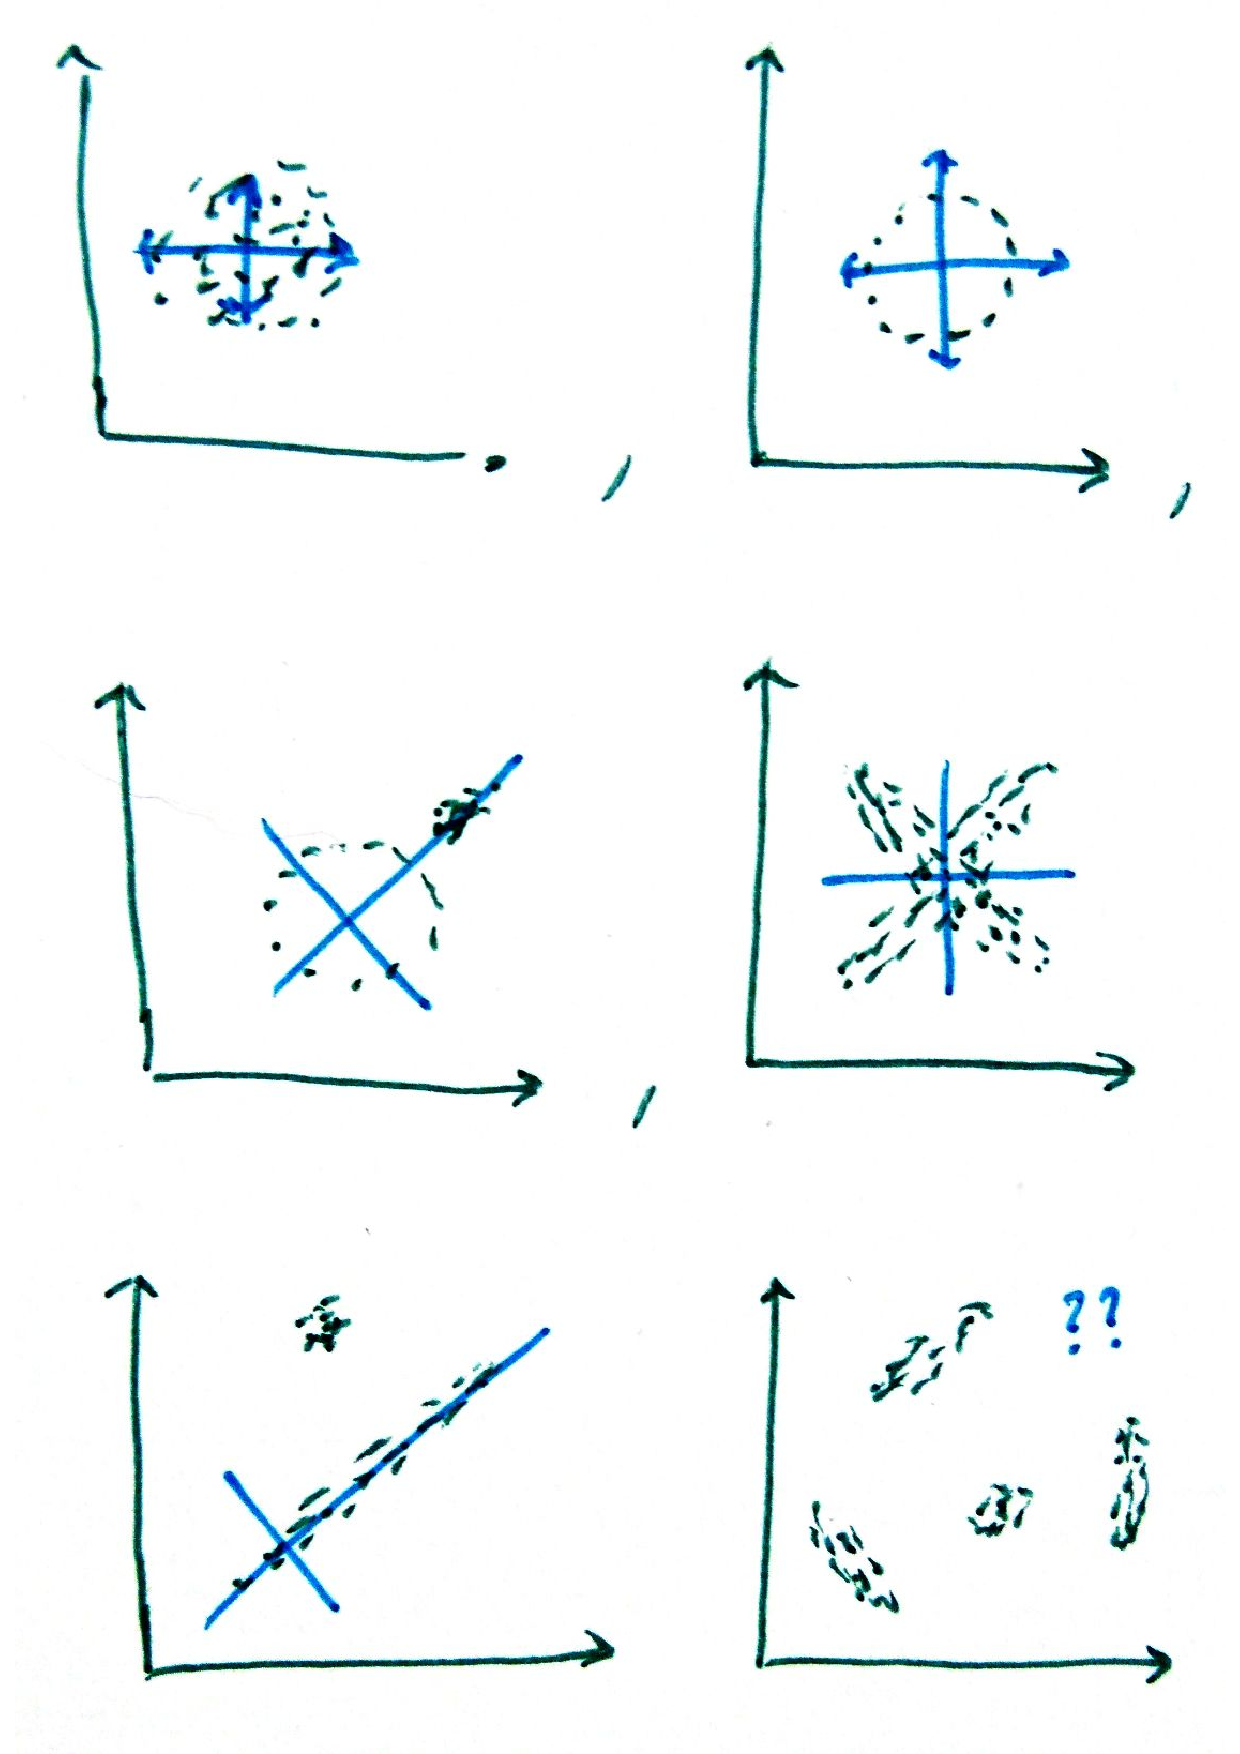
\includegraphics[width=0.8\columnwidth]{figures/pca-examples.pdf}
    \label{fig:pca-examples}
    \caption{Unterste Zeile: Links nicht korrekt, Achse ist an falscher Stelle. Rechts kein sinnvolles Ergebnis.}
\end{figure}



\subsection{Begriffe}

\subsubsection{Clustering vs. Classification vs. Association Rules}

\begin{definition}[Classification] Die einzelnen Klassen sind im Voraus zur Analyse bereits definiert. Versuche, Daten-Objekte den vordefinierten Klassen \textit{zuzuordnen}.
\note{zB Studenten, Angestellte, Professoren, versuche dann, Personen einzuordnen.}
\end{definition}

\begin{definition}[Clustering] Die \textit{Definition} der einzelnen Klassen ist im Vorfeld nicht bekannt. Versuche, Gruppierungen in Daten-Menge zu finden.
\note{zB finde hochgradig aktive Internet-Nutzer: Clustere nach Datenvolumen und Zeit online; identifiziere Zielgruppen für Handytarife}
\end{definition}

\begin{definition}[Association Rules] Quasi Clustering von Bitvektoren (jd. kodiert einen "Einkaufswagen") bzw. von Potenzmengen, suche ähnliche Teilmengen. \note{Habe idR gegeben eine Form von Warenkorb, d.h. Dinge, die miteinander in Beziehung stehen. Versuche, Regeln zu finden wie "$A$ ist gegeben, dann ist auch $B$ sehr wahrscheinlich"; zB Beziehungen zwischen Produkten in Supermarkt}.
\end{definition}

\begin{definition}[Outlier Analysis] 
       Genaugenommen Sub-Problem von Clustering. \note{Versuche, Outlier zu identifieren, zB Verbrecher}
\end{definition} 

\subsubsection{False positives vs. false negatives}

\begin{definition}[False positive] 
    Algorithmus klassifiziert Objekt als zugehörig, ist es aber in Wirklichkeit nicht.
\end{definition} 

\begin{definition}[False negative] 
       Algorithmus klassifiziert Objekt als \textit{nicht} zugehörig, dabei ist es tatsächlich zugehörig.
\end{definition} 

\subsubsection{Supervised vs. unsupervised learning}

\begin{definition}[Supervised learning] 
    Habe ``Trainings''-Daten gegeben von denen die Klassen bekannt sind. Nutze
    diese als Grundlage für Algorithmus. \note{Beispiel: Neuronale Netze, Naive
      Bayes Classifier, Decision Trees}
\end{definition} 

\begin{definition}[Unsupervised learning] 
  Es wird nicht auf Trainingsdaten zugegriffen. \note{Beispiel: Clustering-Algorithmen}
\end{definition} 

\subsubsection{Classification vs. Prediction}

\begin{cptitemize}
\item \textbf{\inlinedef{Classification}}: Will Klassen-Attribut für neue Werte
  vorhersagen
\item \textbf{\inlinedef{Prediction}}: Sage beliebigen numerischen Wert vorher.
  \note{zB Regression.}
\end{cptitemize}


\subsubsection{Eager vs Lazy Learners}
\begin{definition}[Lazy Learning]
  Berechnung/Generalisierung wird erst dann angestellt, wenn Ergebnis (zB Klasse für Objekt)
  abgefragt wird (\note{zB $k$-nearest neighbour})
\end{definition}
\begin{definition}[Eager Learning]
  Generalisierung wird bereits im Vorhinein durchgeführt (\note{zB Neuronale
    Netze, SVM})
\end{definition}
\section{Classification}

\subsection{Evaluation of Classifiers}
\begin{cptitemize} 
        \item \textbf{Speed}: \note{DecTrees, NNs Aufbau schwierig, Anwendung einfach. DecTrees aufbauen idR auch kein Problem heute.}
        \item \textbf{Robustness}: Algorithmus soll auf unbekannten Daten ja auch funktionieren.
        \begin{cptitemize} 
                 \item Was geschieht bei sich widersprechenden Datensätzen? (\inlinedef{contradictory examples}) 
                 \item Wie ändert sich Ergebnis, wenn Datensätze hinzugefügt oder weggelassen werden?
         \end{cptitemize}  
       \item \textbf{Scalability}: Komplexität; Dauer, Modell aufzubauen. \note{NNs idR nicht gut skalierbar da Trainingsaufwand hoch -- Ausführung geht allerdings schnell und Genauigkeit recht hoch.}
       \item \textbf{Interpretierbarkeit}: Nachvollziehen, wie Entscheidung zustande kam; Vertrauen in Ergebnis/Algorithmus.
\end{cptitemize} 

\subsubsection{Validation} todo
\subsubsection{Accuracy \& Error} todo
\subsubsection{Precision \& Recall} todo

\subsection{Beispiele für Classifier}
\begin{cptitemize} 
       \item Kreditwürdig oder nicht?
       \item Spam -- Ja/Nein?
       \item Klassifizierung von Text -- Sport/Politik/...?
       \item Wahl-o-mat
 \end{cptitemize}  

\subsection{Decision Trees}

\subsubsection{Konstruktion} 

\begin{cptenumerate} 
      \item Finde ein Attribut, nach dem der Datensatz ``am Besten'' aufgeteilt werden kann
      \item Nehme diesen Knoten als Wurzel, für jede Ausprägung des Attributs erzeuge ein Kind
      \item Wiederhole iterativ bis Abbruchkriterium erreicht (zB gewünschte
        Reinheit eines Blattknotens).
      % \item Wähle eine Attribut als Wurzel
      % \item Für jede Ausprägung stecke Daten in jwlige Kinder
      % \item Repeat via 2.
      % \item Wenn alle Trainingsdaten unter einem Knoten derselben Klasse zugeordnet sind, so stoppe.
\end{cptenumerate}

\note{Konstruktion ist also typischer Divide \& Conquer-Algorithmus}
\textwidthimage{figures/decision-tree-ex.png}{Zu treffende Entscheidung: Soll Kredit gewährt werden?}

\subsubsection{Wahl des Split-Attributs} 
Möchte möglichst bald erreichen, dass Attribute unterhalb eines Knotens nur dieselbe Klasse enthalten. Suche also ein Maß der "Purity" und stelle dann für jeden möglichen Split den "Information Gain" fest. Hierfür gibt es zwei Maße: \textit{Information Gain} und \textit{Gini Impurity}.

\subsubsection{Information Gain \& GainRatio}
\newcommand{\info}{\text{\textit{info}}}
   \newcommand{\gain}{\text{\textit{gain}}}
\begin{enumerate}
   
   \item Berechne ``Reinheit'' von aktuellem Knoten als 
   $$\info(D) := - \sum_{i=1}^{m} p_i \log_2(p_i)$$
   für $m$ Klassen wobei $p_i$ Anteil der Tupel mit Klasse $i$. \note{Klein ist rein}.
% 
   \item Für jedes Attribut $A$ in D, berechne 
   $$\gain(A) := \info(D) - \info_A(D)$$
   wobei
   $$ \info_A(D) := \sum_{j=1}^{v} \frac{\abs{D_j}}{\abs{D}} \cdot \info(D_{A,j}) $$
   mit $D_j$ als Menge der Tupel mit Ausprägung $j$ von Attribut $A$.
   % 
   \item Wähle Attribut mit höchstem $\gain$ für Split. Jede Ausprägung des gewählten Attributs erzeugt also ein neues Kind.
   % 
   \item Rekursiv weiter bis verbleibende Tupel alle in selber Klasse oder anderes Abbruchkriterium erreicht.
\end{enumerate}

Bei numerischen Attributen prüfe alle möglichen Aufteilungen zwischen zwei diskreten Werten auf ihren \textit{information gain} (möglicherweise sehr aufwendig).

\paragraph{Zu beachten}
Bei im Extremfall für jedes Tupel individuelle Attribute (zB \textit{uniqueID}) sollten diese entweder weggelassen werden, oder \textit{GainRatio} angewandt werden (dieser wäre dann sehr klein).

\paragraph{GainRatio}
\newcommand{\gainratio}{\text{\textit{gainRatio}}}
\newcommand{\splitinfo}{\text{\textit{splitInfo}}}
Teile den ursprünglichen information gain durch den Informationsgehalt des Attributs.
$$
   \gainratio(A) = \frac{\gain(A)}{\splitinfo(A)}
$$
$$
   \splitinfo_A(D) = - \sum_{j=1}^{v} \frac{\abs{D_j}}{\abs{D}} \cdot \log_2 \left(\frac{\abs{D_j}}{\abs{D}} \right)
$$
Wähle höchsten.





\subsubsection{Gini Impurity}
\newcommand{\gini}{\text{\textit{gini}}}

\paragraph{Idee} Mache lediglich binäre Splits. Identifiziere Teilmengen von
Ausprägungen, sodass binärer Split auf zugehörigkeit zu Teilmenge
(\textit{subset-split}) möglichst rein.

% Prüfe bei einem Attribut mit diskreten Ausprägungen $A = \{a_1, a_2, ..., a_v\}$ jede Teilmenge $\mathcal{P}'(A) := \mathcal{P}(A) \backslash A, \emptyset$ auf Tauglichkeit

% \begin{align*} 
%    \gini(D) = 1 - \sum_{i \in \text{Classes}} p_i^2
% \end{align*} 
% Wobei $p_i$ Anteil von Klasse $i$.
% Gewichtete Summe der Impurity von jeder resultierenden Partition
% \begin{align*} 
%     \gini_A(D) := \sum_{j \in \mathcal{P}(A)} \frac{\abs{D_j}}{\abs{D}} \cdot \gini(D_j) 
% \end{align*} 
% \note{Bei ledigl. zwei Klassen, zB Yes/No ist $\mathcal{P}'(A) = \{\{Yes\}, \{No\}\}$}

% Die Verminderung an Impurity bei Split an $A$ ist dann gegeben durch:
% \newcommand{\ginigain}{\text{\textit{giniGain}}}
% \begin{align*} 
%      \ginigain(A) = \gini(D) - \gini_A(D)
% \end{align*} 
% Wähle kleinstes $\gini_A$, maximiert den $\ginigain$.


\begin{enumerate}
\item Berechne $\text{gini}(D) := \sum_{c \in \text{Classes}} {p_c}^2$
\item Für jedes Attribut $A$
  \begin{enumerate}
  \item Berechne bestmöglichen $\text{GiniGain}(A)$ erreichbar durch einen
    subset-Split $a$.
    \begin{align*}
     \text{giniGain(A)} := \text{gini}(D) - \min_{A \in \text{Attribute}} \min_{a \in \mathcal{P}(A)} \{ \text{gini}_a \}
    \end{align*}
    Überprüfe dafür alle möglichen subset-splits bzgl. $A$. Sei $a
    \in \mathcal{P}(A)$. Dann
    \begin{align*}
      \text{gini}_a := \frac{\abs{D_a}}{\abs{D}} \text{gini}(D_a)
       + \frac{\abs{\overline{D_a}}}{\abs{\overline{D}}} \text{gini}(\overline{D_a})
    \end{align*}, wobei $D_a$ Menge der Datentupel mit Ausprägung $a$ von
    Attribut $A$ und $\overline{D_a} := D \backslash D_a$.
    \note{gewichtete Summe über resultierende Blätter bei diesem (binären) Split.}
  \end{enumerate}
\end{enumerate}


\paragraph{Zu beachten} Nur binäre Splits 





\subsubsection{Pruning}
Overfitting vermeiden, Baum soll nicht zu groß werden. Standard-Algorithmus wie gegeben würde immer overfitten.

\begin{definition}[Pre-Pruning] lege Abbruchkriterien fest: 
   \begin{cptitemize} 
     \item \textbf{\inlinedef{Minimal Support}}: Minimale Anzahl von Datentupeln in einem Blatt
     \item \textbf{\inlinedef{Minimum Confidence}}: Minimaler Anteil von größter Klasse in Knoten \note{(zB {Ende, falls 95 \%  Ja})}
   \end{cptitemize} 
\end{definition} 

\begin{definition}[Post-Pruning] modifiziere fertigen Baum:
\begin{cptitemize} 
      \item Fasse Knoten zusammen wenn Fehler bei Crossvalidation zu groß wird
      \item Maß für "Cost Complexity" für Entfernen von Teilbäumen.
 \end{cptitemize}  
\end{definition} 

\subsubsection{Diskussion}
\begin{itemize}
         \advantageit Leicht nachzuvollziehen, gute Interpretierbarkeit
         \advantageit Kann numerische und kategorische Daten handhaben
         \advantageit Robust
         \advantageit Schnell aufzubauen
         \disadvantageit Wiederholung von Splits an gleichem Attribut in
         unterschiedlichen Teilbäumen
         \disadvantageit Große Bäume sind schwer nachzuvollziehen
         \disadvantageit Overfitting
\end{itemize}



\subsection{Naive Bayes Classifier}

Gibt nicht lediglich eine Klasse an sondern Wahrscheinlichkeiten, mit welcher das Tupel zu jeder Klasse gehört.

\renewcommand{\vec}[1]{\boldsymbol{#1}}
\newcommand{\hypoth}{H}

\paragraph{Herleitung} 
   Sei $\vec{x} = (x_1, x_2, ..., x_k)$ ein Datentupel bzw. das Ereignis, dass
   das momentan betrachtete Tupel genau so aussieht. Sei $C_i$ das Ereignis,
   dass ein besagtes Tupel in Klasse $i$ liegt. Sei $P(C_i|\vec{x})$ die
   Wahrscheinlichkeit, dass das Tupel in $C_i$ liegt, gegeben, dass es wie
   $\vec{x}$ aussieht. (Dann ist $P(\vec{x}|C_i)$ die Wsl., dass ein Tupel wie
   $\vec{x}$ aussieht, gegeben, dass es in Klasse $C_i$ liegt.)
   
   Bayes' Theorem besagt:
   \begin{align*} 
       P(C_i|\vec{x}) = \frac{P(\vec{x}|C_i) \cdot P(C_i)}{P(\vec{x})}
   \end{align*} 
   \note{Folgt aus Definition von Conditional Probability}.

   Für die Klassifizierung ist der Zähler irrelevant, da die Klasse $i$ gewählt wird, für die $P(C_i|\vec{x})$ am größten ist und der Zähler nicht von $C_i$ abhängt.

   Weiterhin ist $P(C_i)$ als für alle Klassen gleich angenommen (sofern nicht bekannt). Es dreht sich also nur noch um $P(\vec{x}|C_i)$.

   Unter Annahme, dass alle $P(x_i | C)$ voneinander unabhängig sind, können wir schreiben:
   \begin{align*} 
       P(\vec{x}|C_i) = P(x_1|C_i) \cdot P(x_2|C_i) \cdot ... 
   \end{align*} 
   Dieser Wert ist bekannt: Anzahl der Tupel mit Klasse $C_i$, die den Wert $x_k$ für das entsprechende Attribut haben, geteilt durch die Gesamtzahl der Tupel von Klasse $C_i$.


\paragraph{Vorgehen} Für ein gegebenes Tupel $\vec{x}$
\begin{enumerate} 
   \item Für alle Klassen $i$: 
   \begin{enumerate} 
      \item Berechne $P(C_i)$ 
      \item Berechne $P(\vec{x}|C_i)$ für jedes Attribut von $\vec{x}$ unter
        Verwendung von $P(\vec{x}|C_i) = P(x_1|C_i) \cdot P(x_2|C_i) \cdot ...
        $. Dabei ist
        \begin{align*}
          P(x_j|C_i) := \frac{P(x_j \cap C_i)}{P(C_i)} 
        \end{align*}
      \item Berechne $P(\vec{x}|C_i) \cdot P(C_i)$
    \end{enumerate}
   \item Weise Wahrscheinlichkeiten je Cluster zu, bzw. wähle Klasse mit höchstem Wert für $P(\vec{x}|C_i) \cdot P(C_i)$
\end{enumerate} 

\paragraph{Zu beachten}
\begin{cptitemize} 
   \item Wenn eines der $P(x_j|C_i)$ gleich 0 ist (d.h. wenn es kein einziges entsprechendes Beispiel in den Trainingsdaten gibt) ist das ganze Produkt gleich 0. Abhilfe: weglassen.
   \item \textbf{Annahmen}
     \begin{itemize}
     \item Jede Ausprägung eines Attributs ist unabhängig von Ausprägungen der
       anderen Attribute. \note{Jedes der Attribute trägt unabhängig von den
         anderen zur Zugehörigkeit der Klasse bei, unterschlägt mögliche
         Korrelationen zwischen Attributen.}. Falls es
       Korrelationen/Abhängigkeiten zwischen Attributen gibt \note{(wie zB
         Raucher/Lungenkrebs, Alter/Einkommen)}, so werden diese hier nicht
       genutzt. \note{zB Raucher, Lungenkrebs, Herzprobleme, ...}
       \item $P(C_i)$ (class prior probabilities) werden, insofern nicht
         bekannt, als pw. gleich angenommen.
     \end{itemize}
\end{cptitemize}  


\subsubsection{Bayesian Belief Networks}


\pagebreak
\subsection{Support Vector Machines}
Idee: Finde Hyperplane in Raum, die Klassen bestmöglichst trennt.

\begin{definition}[Support Vector]
  Trainings-Datenpunkte, die genau auf den Rändern der bestmöglichst trennenden
  Hyperplane liegen. Hierbei bedeutet ``bestmöglichst trennen'': Mit dem größten
  kürzesten Abstand zu einem Trainings-Datenpunkt.
\end{definition}

\begin{cptitemize}
\advantageit Findet immer globale Lösung
\advantageit wenig anfällig für Overfitting, da Ergebnis nur basierend auf den
Support Vectors
\advantageit Skaliert gut mit hochdimensionalen Daten da Komplexität von Anzahl
der Support Vectors abhängt und nicht von Anzahl Dimensionen.
\advantageit kann auch für Prediction genutzt werden
\advantageit Gute Accuracy.
\disadvantageit langsames Training
\disadvantageit Modell ist schwer interpretierbar.
\disadvantageit Gute Ergebnisse oft erst mit \textit{Kernel Trick}.
\end{cptitemize}

\subsubsection{Non-linear SVMs} 
Überführe Eingabedaten in höherdimensionalen Raum (mittels \textit{Kernel
  function}) und finde dort eine trennende Hyperplane. Deren Oberfläche trennt
dann die Datenpunkte im ursprünglichen Raum.

\begin{cptitemize}
\disadvantageit welches Mapping / Kernel ist am Besten geeignet?
\end{cptitemize}


\subsection{Neural Networks}

\begin{definition}[Multilayer Feed-Forward Neural Network] besteht aus
  \begin{cptitemize}
    \item \textit{Input Layer} (normalisiert auf $[0,1]$)
    \item Einem oder mehreren \textit{Hidden Layers}
      \item Gewichteten Kanten zwischen Knoten (falls \textit{fully-connected
          NN} sind alle Knoten aus einem Layer mit allen aus dem nächsten
        Verbunden)
        \item Aktivierungsfunktionen für jeden Knoten.
  \end{cptitemize}  
\end{definition}

\begin{definition}[Backpropagation]
\begin{cptenumerate}
\item Initialisiere Gewichte (zB zufällig)
\item Propagiere Input nach vorn
  \item Stelle Fehler fest, propagiere Fehler zurück, passe Gewichte an um
    Fehler zu minimieren
    \item Wiederhole bis keine/kaum Verbessung.
\end{cptenumerate}
\end{definition}

\begin{definition}[Learning Rate]
  Faktor aus $[0,1]$ für Änderung in Gewicht bei Backpropagation. Vermeide
  feststecken in localem Maximum. Zu niedrig eingestellt: Training konvergiert
  sehr langsam; zu hoch eingestellt: Oszilliert zwischen nicht ausreichenden Lösungen.
\end{definition}

\begin{cptitemize}
  \advantageit Tolerant ggü. Noise
  \advantageit Gut geeignet für numerische/reellwertige Ein- und \textit{Aus}-gaben
  \advantageit Gut parallelisierbar
  \disadvantageit Lange Trainingsdauer
  \disadvantageit Brauche viele Trainingsdaten
  \disadvantageit Muss Parameter wie zB Netzwerktopologie festlegen
  \disadvantageit Sehr schwer nachzuvollziehen
\end{cptitemize}

\subsection{k-Nearest Neighbour} 
Klasse ergibt sich aus Mehrheitsentscheidung der $k$ nächstliegenden Punkte.
\begin{cptitemize}
  \disadvantageit Noisy oder irrelevante Features/Dimensionen können Ergebnis
  stark negativ beeinflussen (dann liegen womöglich eigentlich ähnliche Punkte in
  dieser Dimension weit auseinander)
  \disadvantageit Wenn Klassen unterschiedlich stark vertreten sind, ist für
  Klassifizierung eines neuen Punktes die besser vertretene Klasse
  wahrscheinlicher (Abhilfe: Gewichtung nach Inversem von Distanz bei Majority Vote).
  \disadvantageit Naive Implementation ist rechenaufwendig.
\end{cptitemize}
Beispiel für \textit{Lazy Learner}.

\pagebreak
\section{Clustering}
\label{sec:clustering-algorithms}
\localtableofcontents

 \paragraph{Güte/Kompaktheit eines Clusterings} 
Innerhalb von Cluster Datenpunkte möglichst ähnlich, zwischen Clustern möglichst verschieden.
 \begin{definition}[TD] 
 Sei $m_c$ der repräsentative Medoid für das Cluster $c$, $d$ eine gegebene Metrik. Definiere für die Güte eines einzelenen Clusters
 \begin{align*} 
     TD(C) = \sum_{p \in C} d(p,m_c) 
 \end{align*}
 \note{Summe über Distanzen aller anderen Punkte aus Cluster zu Medoid}
 und für die Güte eines gesamten Clusterings
 \begin{align*} 
     TD = \sum_{c \in C} TD(c) 
 \end{align*} 
 \note{Summe über alle Cluster-Kosten}
 \begin{cptitemize} 
      \disadvantageit Hängt von Anzahl der Cluster, also gegebenem $k$ ab! \redtag{Beispiel}
 \end{cptitemize} 
 \end{definition} 

 \begin{definition}[Silhouette Coefficient] 
    Sei
    \begin{cptitemize} 
         \item $a(o)$ -- Distanz von $o$ zu Cluster-Repräsentant
         \item $b(o)$ -- kleinste Distanz von $o$ zu Repräsentant von einem anderen Cluster
    \end{cptitemize}. Dann ist die Silhouette von $o$ definiert als:
    \begin{align*} 
       \frac{b(o)-a(o)}{\text{max}\{a(o),b(o)\}} 
    \end{align*} 
    Es gilt $-1 \leq s(o) \leq +1$, höherer Wert ist besser.
 \end{definition} 


\paragraph{Einsatzbereiche} 
\begin{cptitemize} 
   \item Identifikation/Bereinigung von Rauschen in Daten
   \item Reduktion von Daten
   \item Outlier Detection
   \item Verstehen der Daten foo bar anhand der inneliegenden Klassen
   \item Identifizieren von zusammengehörigen Teilmengen/Klassen 
\end{cptitemize} 

\paragraph{Distanzfunktionen} Maß der Ähnlichkeit für zwei Datenpunkte. Entspricht einer Metrik. Beispielsweise:
\begin{cptitemize} 
      \item $lp$-Metrik
      \begin{cptitemize} 
        	 \item $p=1$: \textbf{\inlinedef{Manhattan Distance}} \note{Denke: Nur Schritte entlang Gitter in $x/y$-Richtung, keine Diagonalen}.
        	 \item $p=2$: \textbf{\inlinedef{Euklidean Distance}} \note{Denke: Luftlinie}.
       \end{cptitemize}  
      \item \textit{term frequency} und \textit{inverted document frequency}.
 \end{cptitemize}   

 \subsection{Partitioning Methods}

Vorgehen ist eher \textit{top-down}.

\subsubsection{k-Means Clustering}
\label{k-means}

\paragraph{Parameter}
\begin{cptitemize} 
  	 \item $k$ - Anzahl von Centroiden \note{d.h. Anzahl resultierender Cluster} 
  	 \item (Metrik)
 \end{cptitemize}  

\paragraph{Ausgabe}
\begin{cptitemize} 
	\item Zuweisung für jeden Punkt zu einem Cluster/Centroid (\note{Voronoi-Partitionierung der Datenmenge})
 \end{cptitemize}  

\begin{myalgo}{k-means}
   Wähle $k$ Punkte (zufällig) als initiale Centroide \;
   \Repeat{Keine Verbessung}{
      Weise jeden Datenpunkt dem Cluster zu, wo der entsprechende Centroid am nähesten liegt \;
       Aktualisiere Position der Centroide als Durchschnitt aller momentan zugewiesenen Punkte \;
   }
\end{myalgo}


\begin{minipage}{0.5\columnwidth}
	\textwidthimage{figures/k-means-step1.png}{Schritt 1}
\end{minipage}
\begin{minipage}{0.49\columnwidth}
	\textwidthimage{figures/k-means-done.png}{Fertig}
\end{minipage}

\paragraph{Beurteilung}
\begin{cptitemize} 
  	\advantageit \textbf{Speed}: Schnell ($\mathcal{O}(t \cdot k \cdot n)$) wobei $t$ Anzahl Iterationen.
  	\advantageit Einfach zu implementieren
  	\disadvantageit Benötigt Parameter $k$, d.h. Anzahl Cluster muss vorher bekannt sein.
  	\disadvantageit \textbf{Noise, Outlier}: 
  	\begin{cptitemize} 
  	 	 \item verzerren sehr stark die Berechnung der Durchschnitts-Centroide.
  	 	 \item Noise-Punkte werden auch klassifiziert, keine Unterscheidung zwischen
  	 	 	Daten- und Noise-Punkten
  	\end{cptitemize}
  	\disadvantageit \textbf{Cluster Shape}: Kann nur Cluster identifizieren, die in Voronoi-Partitionierung passen, d.h. kann keine nicht-konvexen Formen erkennen.
  	\disadvantageit Ergebnis abhängig von initaler Wahl der $k$ Centroide, nicht deterministisch
  	\disadvantageit Terminiert lediglich bei lokalem Maximum.
 \end{cptitemize}  


\subsubsection{ISODATA}
Erweiterung von $k$-Means. Cluster können aufgeteilt oder zusammengeführt
werden, falls Constraints überschritten werden.

\paragraph{Parameter}
\begin{cptitemize} 
  	 \item $k$: initiale Anzahl Centroide / Cluster
  	 \item \cd{maxIter} Beschränkung für Anzahl Iterationen
  	 \item \cd{MinPts} Mindestanzahl Punkte für ein valides Cluster
  	 \item \cd{MinDist} Minimale Distanz zwischen zwei Clustern vor merge.
  	 \item \cd{StdDev} Maximale Standardabweichung für Werte in Cluster bevor split.
 \end{cptitemize}  

 \paragraph{Algorithmus} Zunächst ähnlich wie $k$-Means. In Schleife zusätzlich:
 \begin{cptitemize} 
   	 \item Cluster werden \textit{zusammengeführt}, falls
   	 \begin{cptitemize} 
   	  	 \item Größe des Clusters kleiner als \cd{MinPts}
   	  	 \item Zwei Cluster sind einander näher als \cd{MinDist} 
   	 \end{cptitemize} 
   	 \item Cluster werden \textit{getrennt}, falls
   	 \begin{cptitemize} 
   	  	 \item Standardabweichung des Clusters übersteigt \cd{StdDev} \textit{und} Größe des Clusters ist größer als $2 \cdot$ \cd{MinPts}. 
   	 \end{cptitemize} 
  \end{cptitemize}  

\paragraph{Beurteilung}
\begin{cptitemize} 
	\advantageit Kann eine variable Anzahl Cluster erkennen.
  	\disadvantageit Noch mehr Parameter nötig
  	\item cf. $k$-Means.
 \end{cptitemize}  

\myhline

\subsubsection{k-Medoids (PAM, Clarans)}
Um Problem mit Outliern abzuhelfen, nutze statt Durchschnitts-Centroiden etwas anderes.

Im Unterschied zu $k$-Means (i-welche Werte) nutzt $k$-Medoids tatsächliche Datenpunkte als Cluster-Zentren.

\begin{definition}[Medoid] Repräsentant eines Clusters, der am zentralsten gelegen ist in diesem Cluster. Frage, wie Medoid gewählt wird führt zu PAM.
\end{definition} 

\begin{minipage}{0.5\columnwidth}
	\smalltwimg{figures/medoid-bad.png}{Nicht so gut.}
\end{minipage}
\begin{minipage}{0.49\columnwidth}
	\smalltwimg{figures/medoid-better.png}{Besser}
\end{minipage}

\paragraph{Parameter}
\begin{cptitemize} 
  	 \item $k$ -- Anzahl Cluster 
 \end{cptitemize}  

 \paragraph{Vergleich}
 \begin{cptitemize} 
   \disadvantageit Muss $k$ angeben
   \disadvantageit Kann nur konvexe Cluster finden.
\end{cptitemize}  


\myhline

 Nun stellt sich die Frage, wie genau wir Medoide feststellen und Cluster zuweisen. Dafür gibt es verschiedene Herangehensweisen:

\paragraph{PAM} \gray{Paritioning around Medoids} 

\begingroup
\removelatexerror
\begin{algorithm}[H]
   Initalisiere $k$ Punkte als Medoide \;
   Weise jeden Punkt dem Medoid zu, der anhand gegebener Metrik am Nähesten liegt. \;
   \While{Kosten des momentanen Zustands verringen sich}{
      \ForEach{Medoid $m$, Datenpunkt $o$}{
        Tausche $m$ und $o$ \;
        Weise Punkte neu dem nächsten Medoid zu \;
        Berechne neue Kosten \;
         \If{Kosten größer}{
            Mache Tausch rückgängig.
         }
      }
   }
\end{algorithm}
\endgroup

$\mathcal{O}(k(n-k)^2)$ in jeder Iteration.

\paragraph{Clarans} \gray{Clustering Large Applications} 

{Im Prinzip gleich wie PAM, aber:
\begin{cptitemize} 
     \item Es werden nicht alle anderen Punkte als potentielle neue Medoide überprüft sondern es werden 
\end{cptitemize} 
}

Zusätzliche Parameter:
\begin{cptitemize} 
     \item \cd{maxIts} -- maximale Anzahl Iterationen \note{Komplette "Neuversuche" des Algorithmus}
     \item \cd{maxNeighs} -- maximale Anzahl von betrachteten Nachbarn \note{potentiellen Alternativen für einen Medoid} 
\end{cptitemize} 

\begingroup
\removelatexerror
\begin{algorithm}[H]
\tcp{Komplette Neuversuche}
\For{$r$ from $1$ to $\mathit{maxIts}$}{ 
   choose $k$ objects as Medoids \uwave{randomly} \;
   $i \gets 0$ \;
   \While{$i<\mathit{maxNeigh}$}{
      choose randomly a tuple of medoid and non-medoid $(M, N)$ \;
      \If{$TD_{NM} < TD$}{ \tcc{better score after swap}
         $M \gets N$ \tcc{assign new medoid} 
         $TD \gets TD_{NM}$ \tcc{assign new score} 
         $i \gets 0$ \tcc{have to start over with neighbours} 
      }
      \Else{
         $i \gets i+1$ \tcc{proceed} 
      }
   }
   If better, update $TD_{best}$ with $TD$ \;
   Record the current medoids\;
}
\Return current medoids
\caption{Clarans}
\end{algorithm}
\endgroup

\begin{cptitemize} 
     \advantageit Schneller als PAM
     \advantageit \cd{maxIts}, \cd{maxNeighs} schränken Laufzeit ein
     \disadvantageit Mehr Parameter zu wählen
     \disadvantageit Ergebnis hängt von der Sampling-Methode ab 
\end{cptitemize} 

\paragraph{Beurteilung} \gray{k-medoids und Varianten} Im Wesentlichen
ähnlich zu \textit{k-means}.
\begin{cptitemize} 
  	 \item \textbf{Noise, Outlier}: Durch Verwendung von Medoiden
  	 	(echten Datenpunkten) wird Empfindlichkeit ggü Outliern bzw.
  	 	ungleich verteiltem Noise abgeschwächt im Vergleich zu 
  	 	\textit{k-means} (\note{cf \ref{k-means}}).
  	 \item \textbf{Cluster Shape}: Nur konvexe Cluster
  	 \item \textbf{Dichte}: Unterschiedl. dichte Cluster verzerren
  	 ebenfalls Zuweisung der Centroide (\note{nach Def. von $TD$, wenn ich es
  	 richtig verstehe}).
 \end{cptitemize}  

\myhline

\subsubsection{Expectation Maximisation}

\begingroup
\removelatexerror
\begin{algorithm}[H]
   \caption{Expectation Maximisation}
   Randomly position $k$ Gaussian distributions \;
   Assign data points to the cluster distributions (functions) \;
   Re-estimate mean and variance of the distributions \;
   Repeat until no improvement \;
\end{algorithm}
\endgroup

\begin{cptitemize} 
 	 \item \textbf{Noise, Outlier}: können Bild verzerren
 	 \item \textbf{Cluster Shape}: Lediglich konvexe Cluster
 	 \item \textbf{Dichte}: Kann gut mit unterschiedl. dichten Clustern
 	 umgehen.
 	 \item \textbf{Hierarchie}: Keine.
 	 \advantageit Liefert Wahrscheinlichkeit für Klasse,
 	 Mehrdeutigkeiten sind somit sichtbar.
\end{cptitemize} 

% \columnbreak

\subsection{Hierarchical \& Linkage-based methods}

\textwidthimage{figures/linkage-dendro.png}{liefert Dendrogramm. (Hierarchisches Clustering)}

\begin{cptitemize} 
   \advantageit \textbf{Parameter}: Keine
   \advantageit \textbf{Cluster Shape}: beliebig, solange gut
   dichte-separiert.
   \advantageit \textbf{Hierarchie}: Kann hierarchische
   Cluster-Strukturen abbilden
   \disadvantageit \textbf{Noise}:
   \begin{cptitemize} 
    	 \item  Noise-Punkte werden nicht als solche erkannt
    	 \item Noise-Punkte können Dendrogramm unübersichtlich machen
   \end{cptitemize} 
   \disadvantageit Muss immernoch Clustering aus Dendrogramm herauslesen.
   \disadvantageit \textbf{Speed}: Ineffizient, in $\mathcal{O}(n^2)$. 
   \textit{Centroid Linkage} noch am schnellsten.
\end{cptitemize}

\begingroup
\removelatexerror
\begin{algorithm}[H]
   \caption{Linkage-based Clustering}
   Jeder Datenpunkt ist zunächst einzelnes Cluster. Berechne Distanzen zwischen jedem Paar von Clustern. \note{$\mathcal{O}(n^2)$} \;
   In jedem Schritt werden die beiden Cluster mit der minimalen Distanz vereint. \note{$\mathcal{O}(n)$}\;
   Berechne Distanzen neu. \;
   Ende, falls nur noch ein Cluster vorhanden.
\end{algorithm}
\endgroup

\begin{definition}[BIRCH]
  Nutze Zusammenfassungen (\textit{clustering features}, \inlinedef{CF}) von
  statistischen Werten um Mikro-Cluster zu beschreiben. Bei Merge von zwei
  Mikro-Clustern kann ein neues \textit{CF}-Tupel einfach aus den direkten
  Kindern berechnet werden.
\end{definition}

\begin{definition}[CF-Tree]
  \begin{cptitemize}
  \item (Ähnlich wie B-Baum) Einschränkung vom Anzahl Schlüsseln in Knoten
    \item Füge nacheinander \textit{CF}-Tupel ein, baue so Baum auf. Dabei darf
      Durchmesser (bezüglich eines Distanzmaßes) aller Punkte in einem Blattknoten nicht einen Schwellwert überschreiten.
    \end{cptitemize}
    Findet auf diese Weise konvexe Cluster.
\end{definition}

\begin{definition}[Linkage-based Clustering]
  Fasse iterativ zwei Punkte mit minimaler Distanz zusammen, baue so ein
  Dendrogramm auf.
  \begin{cptitemize}
    \advantageit keine Parameter
    \advantageit findet auch nicht-konvexe Cluster
    \disadvantageit muss passendes Distanzmaß finden
    \disadvantageit Ergebnis unklar falls nicht klar dichte-separiert
  \end{cptitemize}
\end{definition}

\begin{definition}[Method of Wishart]
  Define a density around data points. All other points are regarded as noise
  and not considered for linkage-based clustering later on.
\end{definition}

\paragraph{Mögliche Distanzmaße}:

\begin{cptitemize} 
     \item \textbf{\inlinedef{Single Linkage}}: \gray{Minimum}
     $$d(C_1, C_2) = \min_{p \in C_1, q \in C_2} ( d(p,q) ) $$ 
     \begin{cptitemize} 
            \advantageit Gut auch bei zB Snake Data wenn doch noch dichtesepariert.
             \disadvantageit Noise-Punkte können "Brücke" bilden und somit Dendrogramm schwer interpretierbar machen (\note{cf Educlust})
     \end{cptitemize} 
     \item \textbf{\inlinedef{Complete Linkage}}: \gray{Maximum}
     $$d(C_1, C_2) = \max_{p \in C_1, q \in C_2}(d(p,q))$$
     \begin{cptitemize} 
       \disadvantageit Nicht gut bei nicht-konvexen verschlungen Clustern \note{zB Snake Data}  
     \end{cptitemize} 
     \item \textbf{\inlinedef{Centroid Linkage}}: \gray{Durchschnitt}
     $$d(C_1, C_2) = d( \text{mean}(C_1), \text{mean}(C_2) )$$
     \begin{cptitemize} 
       \disadvantageit Nicht gut bei nicht-konvexen verschlungen Clustern \note{zB Snake Data} da eher runde Gruppen zusammengefasst werden.
     \end{cptitemize} 
     \item \textbf{\inlinedef{Ward's Method}} \note{Error sum-of-squares}: $\sum D(x, \mu)^2$
\end{cptitemize} 

\smalltwimg{figures/single-linkage.png}{Single Linkage}
\smalltwimg{figures/complete-linkage.png}{Complete Linkage}
\smalltwimg{figures/centroid-linkage.png}{Centroid Linkage}



\subsection{Density-based Methods}

\subsubsection{Definitions}

\begin{definition}[Core Object] 
     Objekt $o \in O$ ist \inlinedef{Kern-Objekt} in O gdw.
$$\abs{N_\varepsilon(o)} \geq \mathit{MinPts}$$, wobei $\abs{N_\varepsilon(o)} = \{\, o' \in O \,\,|\,\, d(o,o') \leq \varepsilon\} $ (Beachte: $o \in N_\varepsilon(o)$) 
\end{definition} 

\begin{definition}[directly density reachable] 
     $p \in O$ ist \inlinedef{direkt dichte-erreichbar} von $q \in O$ (w.r.t $\varepsilon$ und $\mathit{MinPts}$) gdw.
\begin{cptitemize} 
     \item $p \in N_\varepsilon(q)$ 
     \item $q$ ist Kern-Objekt
\end{cptitemize} 
\end{definition} 

\begin{definition}[density reachable] 
     $p$ ist \inlinedef{dichte-erreichbar} von $q$, falls es eine Kette von direkt dichte-erreichbaren Objekten zwischen $q$ und $p$ gibt. 
\end{definition} 

\begin{definition}[density-connected] 
     $p$ und $q$ sind \inlinedef{dichte-verbunden}, wenn beide von einem dritten Objekt $o$ dichte-erreichbar sind. 
\end{definition} 

\begin{definition}[border object] 
     $o \in O$ ist \inlinedef{Rand-Objekt} in O gdw.
\begin{cptitemize} 
     \item $o$ ist kein Kern-Objekt
     \item $o$ ist dichte-erreichbar von einem anderen Objekt $p$ 
\end{cptitemize}  
\end{definition} 

\begin{definition}[Cluster] w.r.t. $\varepsilon$ $\mathit{MinPts}$ ist eine nichtleere Teilmenge von $O$ mit
\begin{cptitemize} 
     \item \textbf{Maximalität}: $$
      \forall p,q \in O: p \in C ~~ \land ~~ p \text{ density-reachable from } p ~~ \Rightarrow ~~ q \in C
     $$
     \item \textbf{Konnektivität}: $$
      \forall p,q \in C: p \text{ ist dichte-verbunden mit } q
     $$
\end{cptitemize} 
\end{definition} 

\begin{definition}[Clustering] besteht aus...
     \begin{cptitemize} 
           \item  Menge aller Cluster
           \item Menge von Noise-Punkten (die, die keinem Cluster zugewiesen wurden.)
      \end{cptitemize}  
\end{definition} 



\smalltwimg{figures/directly-density-reachable.png}{directly density reachable}

\smalltwimg{figures/density-reachable.png}{density reachable}

\smalltwimg{figures/density-connected.png}{density connected}


\subsubsection{DBSCAN}

\paragraph{Parameter}
\begin{cptitemize} 
      \item $\varepsilon$ -- Radius für Nachbarschaft
      \item \textit{MinPoints} -- Mindestanzahl in Nachbarschaft
 \end{cptitemize} 

\begin{myalgo}{DBSCAN}
   Wähle bisher noch nicht betrachteten Punkt $P$ \;
   Finde alle Punkte, die von $P$ aus dichte-erreichbar sind \;
   \uIf{$P$ ist Kern-Objekt}{
     Erstelle neues Cluster \tcp{mit Punkten}
   }
   \Else{
      Klassifiziere $P$ als Noise \;
      \tcc{Punkte können später noch einem Cluster zugewiesen werden}
   }
   Finde alle von der Nachbarschaft von $P$ aus dichte-erreichbaren Punkte und weise sie dem momentanen Cluster zu. \;
   \If{Ein Punkt $r$ ist Randobjekt}{
      \tcp{Keine Punkte sind von $r$ aus dichte-erreichbar}
      Gehe zu Schritt 1
   }
\end{myalgo}

\begin{itemize} 
   \advantageit Kann gut nicht-konvexe Cluster abbilden (zB Snake Data).
   \advantageit Muss Anzahl Cluster nicht vorgeben.
   \advantageit Kann Noise unterscheiden.
   \disadvantageit Kein gutes Ergebnis falls unterschiedliche Cluster unterschiedlich dicht (\note{bräuchte dann unterschiedl. Parameter})
   \disadvantageit liefert keine Hierarchie
   \disadvantageit Sehr empfindlich ggü. Parametern $\varepsilon$ und \lstinline$minPts$. Beispiel: \todo{todo}
\end{itemize} 

\begin{definition}[k-distance Diagram] hilft beim Finden von $\varepsilon$, $\mathit{MinPts}$: 
      \begin{cptitemize} 
           \item \inlinedef{k-Distanz}: Abstand eines Objektes zu seinem $k$-nächsten Nachbarn.
           \item Faustregel: \textit{MinPts} $\gets k+1$
           \item Falls Cluster und Noise gut dichtesepariert, so ergibt sich in Plot zwischen $k$-Distanz und Objekten ein Knick, wähle diese Distanz als $\varepsilon$.
           \disadvantageit Falls nicht gut dichtesepariert /hierarchisch ergibt sich auch kein gut erkennbarer Knick in Plot (\note{$\rightarrow$ OPTICS})
      \end{cptitemize} 
      \smalltwimg{figures/k-distance-diag.png}{k-distance diag.}
\end{definition} 

\subsubsection{OPTICS}
\note{variable epsilons}
\note{liefert reachability-plot}

\textwidthimage{figures/reachability-plot.png}{Reachability Plot}

\begin{definition}[Core Distance] \note{wird in EduClust, falls
    undefiniert, auf den gleichen Wert als die CoreDist gesetzt.}
     \begin{align*} 
          & \mathit{CoreDistance_{\varepsilon, \mathit{minPoints}}}(o) = \\
          & \hspace{1em} \begin{cases} 
              \mathit{MinPtsDistance}(o) & \text{iff $o$ is core object} \\
              \mathit{undefined} & \text{else}
          \end{cases} 
      \end{align*}  
      wobei \textit{MinPtsDistance} der Radius, sodass \textit{MinPts} viele Punkte inneliegend. Ist \textit{undefined} wenn kein Kern-Objekt.
\end{definition} 

\begin{definition}[Reachability Distance] \note{In OPTICS ist $o$ das
    ``vorherige'' Objekt und $p$ der neu hinzukommende Punkt. In EduClust wird
    bei ``Schritt zu Noise-Punkt'', d.h. neuer Iteration der \cd{while}-Schleife
  trotzdem der zuletzt betrachtete Punkt für \textit{ReachabilityDist}
  herangezogen (obwohl kein Kernobjekt), $CoreDist$ wird dann dem gleichgesetzt da eigentlich undefiniert.}
\begin{align*} 
       & \mathit{ReachabilityDist_{\varepsilon, \mathit{minPoints}}}(p,o) = \\
       & \hspace{1em} \begin{cases} 
            \text{max}\{ \mathit{~CoreDist(o)},~ d(o,p) ~ \} & \text{iff $o$ is core object} \\
            \mathit{undefined} & \text{else}
       \end{cases} 
\end{align*}
\end{definition} 


\begin{myalgo}{OPTICS}
   Set all points as unprocessed. \;
   Insert random unprocessed point into \textit{ControlList} \;
   \While{ControlList not empty}{
      Select first element $o$ from ControlList \;
      determine $N_{\varepsilon}(o)$ and $\mathit{CoreDist}(o)$ \;
      set $o$ as processed \;
      write $(o, \uwave{\mathit{rdist}}, \uwave{\mathit{cdist}})$ to file\; 
      \tcp{these are technically undefined for very first elem}
      \If{$o$ is core-object}{
         \tcp{Falls Kernobjekt: schaue Nachbarn an}
         \ForEach{$p \in N_{\varepsilon}(\text{\uwave{$o$}})$ not yet processed}{
            \textit{rdistO} $\gets$ $\mathit{ReachabilityDist}(p,\text{\uwave{$o$}})$ \;
            insert $(p, \mathit{rdistO}, \mathit{cdist})$ into \textit{ControlList} or update if $rdistO$ is smaller.
         }
      }
   }
\end{myalgo}
\note{Erzeugt praktisch lediglich Plot aus Reachability Distance und Core Distance}

\smalltwimg{figures/optics-example.png}{Möglicher Verlauf}

\smalltwimg{figures/reachability-plot-detail.png}{Bei erstem Punkt in neuem
  Cluster ist \textit{Core Distance} niedrig (da Kernobjekt),
  \textit{Reachability Distance} aber hoch, da dies hier die Distanz zum vorher
  betrachteten Punkt ist. -- Bei einem Schritt zwischen zwei Nicht-Kernobjekten
  (neue \cd{while}-Iterationen) wird \textit{R.d} und \textit{C.d} willkürlich
  auf deren Distanz gesetzt.}

\begin{cptitemize} 
   \advantageit Kann $\varepsilon$ interaktiv anpasen
   \advantageit Reachability Plot liefert Informationen über Cluster-Hierarchien
   \disadvantageit Findet selbst keine Cluster, liefert lediglich Reachability Plot
\end{cptitemize} 


\myhline
\subsubsection{DENCLUE}

Jeder Punkt erhält eine \inlinedef{influence function}, die den Einfluss
umliegender Punkte auf ihn angibt (wsl. in Abhängigkeit der Distanz).

Die Summe über die \textit{influence functions} spiegelt die Dichte im Datenraum
wieder (\inlinedef{density function}).

Identifiziere nun \inlinedef{density attractors} (\note{``Spitzen''} der Berge).
$y$ ist zu $x*$ \textit{density-attracted}, falls eine Folge $y, x_1, ..., x*$
existiert sodass die Steigung von $x_{i-1}$ in Richtung $x_i$ geht. Punkte um
einen \textit{density attractor} bilden ein Cluster (siehe unten).

Mit gegebenem Threshold $\zeta$:
\begin{enumerate}
\item \inlinedef{\textbf{Center-defined Cluster}} um $x*$: Punkte, die
  \textit{density-attracted} zu $x*$ sind und wo die \textit{density function}
  nicht unterhalb von $\zeta$ kommt.
\item \inlinedef{\textbf{Arbitrary-Shape Cluster}}: Menge von
  Center-defined Clustern wobei zwischen jedem \textit{density attractor} ein
  Pfad von Punkten mit Dichte-Wert oberhalb von $\zeta$ existiert.
\end{enumerate}

\textwidthimage{figures/denclue.png}{Addition von \textit{influence functions}.}

\pagebreak
\subsection{Beispiele}

\smalltwimg{figures/clustering-example-1.png}{Unklar abgegrenzte Cluster,
Gaußsche Cluster}
\paragraph{k-means} Gutes Ergebnis, Noise-Punkte dazwischen werden aber auch
klassifiziert.
\paragraph{EM} Womöglich wegen Noise kaum erkennbares Ergebnis, da die
Gauß-Kurven sehr ähnlich zueinander werden. Falls $k=3$ gewählt könnten sich die
Cluster mit kleinem Unterschied herausbilden.
\paragraph{Linkage} Cluster sind in Dendrogramm erkennbar, eventuell aber keine
gute Abgrenzung zu finden.
\paragraph{DBSCAN} Keine guten Ergebnisse, da Punkte nicht gut dichtesepariert.
Hängt hier sehr von der perfekten Wahl der Parameter ab (wsl. insbesondere
$\varepsilon$).
\paragraph{OPTICS} Reachability Plot wird nur unklare Abgrenzugen liefern,
manuelles Herantasten an $\varepsilon$ könnte für gegebenen Datensatz gut
helfen, könnte aber auch Overfitting darstellen.
\paragraph{DENCLUE} Hier auch nicht besser als EM.

\newpage

\smalltwimg{figures/clustering-example-2.png}{Cluster verschiedener Dichte}
\paragraph{k-means} Sehr dichtes Cluster würde Zuweisung der Centroide
verzerren, d.h. diese würden alle Stark in Richtung dieses Clusters tendieren.
Im Extremfall würden sich alle Centroide dort sammeln und ein Punkt die
restlichen Cluster abdecken. Mit höherem $k$ wird die Chance erhöht, dass
Centroide in undichtere Cluster fallen, dann eher noch eine Chance mit
Nachverarbeitung.
\paragraph{EM} Gute Ergebnisse insofern $k$ korrekt gewählt da sich Gauß-Kurven
eindeutig in den Clustern konzentrieren und aufsummieren. Noise-Punkte sind klar
unterscheidbar, da dort niedrige Werte.
\paragraph{Linkage} Für dichte Cluster sehr gute Ergebnisse. Noise allerdings
womöglich nicht gut von oberem Ende von Dendrogramm abgrenzbar.
\paragraph{DBSCAN} Sehr gute Ergebnisse für dichte Cluster, mit passender Wahl
von $\varepsilon$ auch das dünne Cluster da noch Unterschied besteht. Treffender
Parameter könnte mit \textit{$k$-distance diagram} wsl. gefunden werden.
\paragraph{OPTICS} Sehr gutes Ergebnis, Abgrenzung zwischen dünnem Cluster und
Noise auffindbar.
\paragraph{DENCLUE} Gleich wie EM?

\newpage

\smalltwimg{figures/clustering-example-3.png}{Snakey Data}
\paragraph{k-means} Kann kein sinnvolles Clustering liefern da $k$-means
lediglich Vornoi-Partitionierung von Raum liefert, hier sind Cluster aber
nicht-konvex.
\paragraph{EM} Kein sinnvolles Ergebnis, da sich die $k$ Gaußkurven irgendwie an
ihr Umfeld anpassen würden. EM kann nur konvexe Cluster erkennen.
\paragraph{Linkage} Gute Ergebnisse, einzelne Cluster am oberen Ende des
Dendrogramms abzulesen.
\paragraph{DBSCAN} Gute Ergebnisse mit richtiger Wahl von $\varepsilon$, \textit{MinPts}
\paragraph{OPTICS} Gute Ergebnisse, Unterscheidung zwischen Clustern erkennbar
in \textit{Reachability Plot}.
\paragraph{DENCLUE} Keine Guten Ergebnisse, kann nur konvexe Cluster.

\newpage

\smalltwimg{figures/clustering-example-4.png}{Hierarchische Cluster}
\paragraph{k-means} Wenn Cluster jeweils ähnlich in Dichte könnte mit passendem
$k$ ein gutes Ergebnis erzielt werden. Bekomme aber keine Informationen über
Hierarchie.
\paragraph{EM} Erkennbar mit passender Wahl von $k$.
\paragraph{Linkage} Gute Ergebnisse, insbesondere hierarchische Struktur
erkennbar.
\paragraph{DBSCAN} Je nach Wahl von Parametern werden second-level-Cluster
entweder als Noise klassifiziert oder alle Punkte beider Ebenen bilden ein
Cluster.
\paragraph{OPTICS} In Reachability-Plot womöglich Hierarchie erkennbar.
\paragraph{DENCLUE} Mit Variante \textit{multi-center-defined cluster} und
richtiger Wahl von $\xi$ könnten dünnere Cluster zusammen mit Spitzen als eines
klassifiziert werden. Mit \textit{single-center-defined cluster} und höherem
$\xi$ hätte man nur die ``Spitzen''.




\pagebreak
\section{Association Rule Mining}
\localtableofcontents


\subsection{Definitionen}

\begin{definition}[Transactions] Sei $T = \{t_1, t_2, ..., t_n\}$ die
\textit{Transaction Database}. Jede Transaktion $t \in T$ stellt ein
itemset dar.
\end{definition} 

\begin{definition}[Support] 
      Anteil von Transaktionen, die ein itemset beinhalten.
      \begin{align*} 
          s(A \rightarrow B) := P(A \cup B)
      \end{align*} 
\end{definition} 

\begin{definition}[Frequent Itemset] Ein itemset $M$ ist
  \textit{frequent/häufig} gdw. $s(M) \geq \mathit{minSup}$ wobei
  $\mathit{minSup}$ manuell festgelegt.
\end{definition} 


\begin{definition}[Confidence] 
     \begin{align*} 
          c(A \rightarrow B) := P(B | A) = \frac{s(A \cup B)}{s(A)}
      \end{align*}  
      \note{Angenommen $A$ wurde gekauft gibt $c$ die Wahrscheinlichkeit an,
        dass auch $B$ gekauft wurde.}
\end{definition} 

\paragraph{Beispiel} 
computer $\rightarrow$ software [$1\%$, $50\%$] \\
\note{Wahrscheinlichkeit, dass beiderseits Computer und Software gekauft wird ist $1\%$. Wsl., dass, wenn Computer gekauft wurde, dann auch Software gekauft wurde ist $50\%$.} \\

Problem: Anzahl möglicher itemsets (alle möglichen Teilmengen) ist zu hoch für
einfache Überprüfung.

\begin{definition}[Apriori-Prinzip] 
  Ein itemset kann nicht häufig sein, wenn eine Teilmenge nicht häufig ist. D.h.
  falls ein itemset nicht häufig ist, muss keine Obermenge davon geprüft werden.
      % \note{Ein itemset kann nur häufig sein, wenn jede Obermenge häufig ist. }
\end{definition} 

\subsection{Algorithmus ohne FP-Tree}
\begin{cptenumerate}
\item Candidate generation
  \item Support determination
\end{cptenumerate}

\begin{myalgo}{Apriori-Algorithm}
   \tcc{Baue sukzessiv größere itemsets aus kleineren, eliminiere jeweils die, die nicht häufig sind.}
   \tcp{$C_k$: Candidate $k$-itemsets}
   \tcp{$L_k$: frequent $k$-itemsets}
   $L_1 \gets $ frequent 1-itemsets  \;
   \For{$k=1$, $L_k \not= \emptyset$, $k++$}{
      $C_{k+1} \gets $ \uwave{candidates generated from} $L_k$ \; \tcp{noch offen, wie diese candidate itemsets effizient generiert werden.}
      $L_{k+1} \gets $ candidates in $C_{k+1}$ \uwave{that are frequent} \; \tcp{Noch offen, wie der \textit{support} eines itemsets effizient festgestellt werden kann.}
   }
   \Return $\bigcup L_k$
\end{myalgo}

\begin{cptitemize}
  \disadvantageit Teuer
  \begin{cptitemize}
  \item viele DB rescans
  \item viele Kandidaten ($2^{n-1}$ mögliche frequent itemsets)
  \item muss Teilmengen betrachten
  \end{cptitemize}
\end{cptitemize}


An zwei Stellen \textit{pruning} (candidate generation, support determination).
je nach aufgabenstellung am ende die rules noch nach minimum confidence filtern.

\subsubsection{Candidate Generation}
finden von $C_k$ mittels $L_{k-1}$.

Annahme: Alle itemsets sind sortiert.
\begin{cptenumerate}
\item \textbf{join} -- Führe $p,q \in L_{k-1}$ zusammen zu $(s_1, s_2, ...,
  s_{k-2}, p_{k-1}, q_{k-1})$, falls sie in den ersten $k-2$ Positionen
  übereinstimmen.
\item \textbf{prune} -- Entferne alle Elemente, die eine $k-1$-Teilmenge haben,
  die nicht in $L_{k-1}$ liegt. \note{Dann ist diese Teilmenge nach
    Apriori-Prinzip nicht frequent}
\end{cptenumerate}

\smalltwimg{figures/candidate-generation-prune-example.png}{Wird entfernt, da
  $(3,4,5) \not \in L_3$}



\subsubsection{Support Determination without FP-trees}
Wie kann der \textit{support} eines Candidate Itemsets $c \in C_k$
bestimmt werden? Dies ist entsprechend obiger Definition die Anzahl
aller Transaktionen, in denen $c$ als Teilmenge vorkommt.

% Sei $t \in T$ eine Transaktion.

\paragraph{Start bei Wurzel} 
\begin{enumerate}
      \item Speichere $C_{k-1}$ als Hash-Tree.
      \item Bestimmte Hashwert $h(\tau_i)$ für alle $\tau \in t$ (einzelne Items)
      \item Suche in entsprechendem Kind weiter.
\end{enumerate}

\paragraph{In Innerem Knoten} 
Innerer Knoten wurde erreicht durch $h(\tau)$
\begin{itemize}
   \item Suche weiter für alle Hashwerte $h(\tau_k)$ mit $k > i$
\end{itemize}
\note{Vorsicht: Es geht hier um alle $\tau_k \in t$, nicht lediglich die
$\tau_i$ mit Hashwert gleich dem momentanen Knoten.}

\paragraph{Bei Blattknoten}
\begin{itemize} 
     \item Für jedes Itemset $X$ in diesem Knoten, teste $X \subseteq
     T$. Falls, so inkrementiere den Support Count.
 \end{itemize}

\paragraph{Beispiel}
.
\textwidthimage{figures/hashtree-supportcount.png}{}
\begin{cptenumerate} 
      \item Hashe separat $1, 3, 7, 9, 12$
      \item In bspweise erstem Knoten auf
      zweiter Ebene erreicht durch $h(\tau_2) = 3$ mache weiter mit
      Hashen von $7, 9, 12 \in t > 3 = h(\tau_2)$
 \end{cptenumerate} 

\paragraph{Diskussion}
\begin{cptitemize} 
  	 \disadvantageit Anzahl der Kandidaten immernoch exponentiell.
  	 \disadvantageit Viele Scans der Datenbank notwendig \redtag{wieso?} 
 \end{cptitemize}  

\subsection{FP-Trees}

\begin{myalgo}{FP-Tree Mining}
	\tcc{Bestimme frequent 1-itemsets durch Abzählen.}
	$L \gets $ frequent 1-itemsets in descending order \;
	\ForEach{$t \in L$ \note{(start from back)}}{
		construct conditional pattern base \;
		draw conditional FP-tree for \textit{cpb} 
		\tcp{branches with insufficient support can be discarded}
		\uIf{tree contains a single path $p$}{
			generate patterns $t \cup \alpha$ where $\alpha$ is a combination of nodes in $p$
			, with support = minimum support count of nodes in combination.
		}
		\Else{
			recurse on tree, concat resulting patterns with $t$.
		}
	}
\end{myalgo}

% \paragraph{Konstruktion, am Beispiel}
% \begin{cptenumerate} 
%        \item Gegebene Transaktionen:
%        \begin{cptenumerate} 
%              \item $\{f,a,c,d,g,i,m,p\}$ 
%              \item $\{a,b,c,f,l,m,o\}$
%              \item $\{b,f,h,j,o,w\}$
%              \item $\{b,c,k,s,p\}$
%              \item $\{a,f,c,e,l,p,m,n\}$
%         \end{cptenumerate}  
%         \item Erster Scan liefert geordnete Liste von $1$-itemsets:
%         $[\underbrace{f,c}_{\text{jwls 4 mal }}, ~~ 
%         \underbrace{a,b,m,p}_{\text{jwls 3 mal}} ~~~~ ]$
%         \item Zweiter Scan: Bilde frequent
%         $1$-itemset-Teilmengen jeder Transaktion absteigend nach
%         support.
%         \begin{cptenumerate} 
%              \item $\{f,c,a,m,p\}$ 
%              \item $\{f,c,a,b,m\}$
%              \item $\{f,b\}$
%              \item $\{c,b,p\}$
%              \item $\{f,c,a,m,p\}$
%         \end{cptenumerate}
%         \item Baue Baum daraus auf, inkrementiere jwls, bzw. lege neuen
%         Ast an.
%   \end{cptenumerate}   

%   \textwidthimage{figures/fptree-example.png}{Noch nicht ganz fertig.
%   Wie gehts weiter?}

% \paragraph{Frequent Pattern Mining}
% \begin{cptenumerate} 
%       \item Für jd. frequent $1$-itemset (item) $m$ bestimme die 
%       \inlinedef{conditional pattern base} 
%       $\{ (p,n) \} $ wobei 
%       \begin{cptitemize} 
%        	 \item $p$ ist prefix-Pfad von $m$
%        	 \item $n$ ist minimaler Support auf Pfad (einschl. $m$)
%       \end{cptitemize}
%       \note{cpb: Unter Voraussetzung von $p$, wie häufig sind
%       Vorgänger?}
%       % 
%       \item Für jd. cond. pattern base (bzgl $m$): Bilde Kombinationen
%       aus $m$ und $p$ die frequent sind.
%       \begin{cptenumerate} 
%        	 \item Nehme Vorgänger von $p$ an Anfang von $cpb$ hinzu
%        	 \item bestimme dessen $cpb$ bis keine mehr übrig.
%        	 \item Resultierendes $p$ ist dann ein frequent pattern.
%       \end{cptenumerate} 
%       \note{
%       D | CAB:1, CA:1, CB:1, C:1 liefert ledigl. das frequent pattern
%       $DC$
%       }
%  \end{cptenumerate}  

\paragraph{Optimierung}
   Kann Teilbäume getrennt bearbeiten. \redtag{todo} Projection etc. 

\paragraph{Diskussion} Only when the support threshold is set very low does
the FP-tree’s ability to compress the dataset degrade. Under these
conditions, the tree becomes bushy, with little node sharing.

\begin{cptitemize}
  \advantageit Schneller als Apriori-Algo
  \advantageit FP-Tree komprimiert Datensatz (enthält nur ``wesentliche''
  Infos). Nicht mehr so gut, falls \cd{MinSupport} klein.
  \disadvantageit Langsam, wenn Daten nicht mehr in Arbeitsspeicher passen.
\end{cptitemize}


 
\pagebreak

\section{Diverses}



\paragraph{Beispiele für Machine Learning} 
\begin{cptitemize} 
      \item Warenkorb
      \item Amazon-Crossellilng
      \item Erkennung von Virus durch Analyse von Datenverkehr 
\end{cptitemize} 


\pagebreak


\pagebreak

\section{Visualisierung}
\localtableofcontents

\subsection{Grundlagen}

\paragraph{Motivation} Weshalb Visualisierung?
Visualisierung ergänzt die statistische Analyse komplementär. Statistische Methoden nicht ausreichend, um alle Muster oder Informationen in Daten zu erkennen. (\note{Beispielsweise können sehr unterschiedliche Datenmengen gleiche statistische Kennwerte besitzen, cf Statosaurus}). 

\paragraph{Visualisation} Datenmengen sind durch einfache Inspektion nicht handzuhaben. Es geht bei Visualisierung darum, die menschliche Wahrnehmung zu unterstützen, bzw. neue Blickwinkel zu ermöglichen. Visualisierung ergänzt die statistische/mathematische Analyse komplementär. \note{Beachte auch: die Verfahren an sich generieren keine Einsicht, erst die Interpretation.}

\begin{definition}[Visualisation] 
       The use of computer-generated, interactive, visual representations of abstract data to amplify cognition.
\end{definition} 

\begin{definition}[Visualisation vs. Visual Analytics] 
  \begin{cptitemize}
  \item \textbf{Visual Analytics}: Visualisierung ist Schnittstelle zwischen
    Analyseprogramm und menschl. Experte, Programm nimmt Expertenwissen auf.
  \item dahingegen \textbf{Visualisierung}: statisches In-/Output, keine
    direkte Interaktion. \inlinedef{Ziele} (nur in eine Richtung, einzelner Schritt):
    \begin{cptitemize}
    \item \textbf{Präsentation} von Daten. Die darzustellenden Fakten sind
      bereits bekannt und es gilt, eine geeignete Visualisierung zu finden um
      diese Fakten zu kommunizieren.
    \item \textbf{Confirmatory Analysis} Gegeben ist eine Hypothese. Führe eine
      zielorientierte Überprüfung durch.
    \item \textbf{Exploratory Analysis} Keine Hypothese gegeben. Versuche durch
      (oft interaktive, indirekte) Exploration der Daten Muster oder Trends zu
      gewinnen.
    \end{cptitemize}
    Vis. kann hier Mittel von Visual Analytics sein (\note{wie ich es verstehe}).
  \end{cptitemize} 
\end{definition}

\begin{definition}[Change Blindness]
  Kleine Änderungen an Bild werden nicht wahrgenommen, insbesondere wenn:
  \begin{cptitemize}
  \item Kein Fokus
  \item weicher Übergang
  \item zwischendrin Ablenkung
  \end{cptitemize}
\end{definition}

\begin{definition}[Pre-attentive Perception] \gray{Pre-attentive processing}
  Information wird ohne bewusste Interpretation wahrgenommen. zB Scatterplot von
  gleichförmigen Glyphen, eine hat dabei eine auffällig andere Farbe.
\end{definition}

\begin{definition}[Similarity Theory]
  \begin{cptitemize}
  \item Suchzeit abhängig, wie leicht Ziel von anderen zu unterscheiden ist
  \item Suchzeit abhängig von unterschiedl. Information ggü. gesamter
    Information
  \item target/non-target-Ähnlichkeit steigt $\Rightarrow$ Suchzeit steigt
    \item inter-non-target-Ähnlichkeit steigt $\Rightarrow$ Suchzeit steigt
  \end{cptitemize}
\end{definition}

\begin{definition}[Gestalt Laws]
  \begin{cptenumerate}
  \item Nähe
  \item Ähnlichkeit
  \item Verbundenheit
  \item Geschlossenheit
  \item Fortsetzung
  \item Symmetrie
  \item Figur/Grund
  \end{cptenumerate}
  Sollten genutzt werden, um Objekte zu gruppieren, Zugehörigkeiten zu
  Verdeutlichen, verschiedene Gruppen voneinander abzugrenzen, ...
\end{definition}

\begin{definition}[Visual Variables]
  \begin{cptitemize}
  \item Position
  \item Shape / Mark
  \item Size (Length, Area, Volume)
  \item Brightness
  \item Hue (Color)
  \item Angle / Orientation
  \item Texture
  \item Motion
  \end{cptitemize}
\end{definition}

\begin{definition}[Interpretation Accuracy of Vis. Var.s] of numerical values
  In dieser Reihenfolge können abgebildete Werte (\textit{mapping} von Daten auf
  visuelle Variablen) mit absteigender Genauigkeit wieder ausgelesen werden:
  \begin{cptenumerate}
  \item Position
  \item Length
  \item Angle, Shape
  \item Area
  \item Volume (3D)
  \item Color, Density
  \end{cptenumerate}
  Dies ergibt sich aus dem Konzept \textit{difference of least noticeable change}.
  \textwidthimage{figures/visvars-ranking.png}{... oder in anderer Ausführung}
  \textwidthimage{figures/munzner-fig5-1.pdf}{cf. Munzner: Data Analysis and Visualisation}
\end{definition}

\begin{definition}[Levels of information]
  Information über...
  \begin{cptenumerate}
    \item \inlinedef{... einzelne Objekte}: zB Welches Auto hat den
      höheren Preis?
    \item \inlinedef{... Gruppen von Objekten}: zB ``Was ist besonders an der
      Marke Audi?'', ``Was passierte in dieser Zeitspanne?''
    \item \inlinedef{... Mengen von Objekten}, d.h. abstrakte, globale Information, wie
      zB ``Zu welcher Jahreszeit und welchen Angeboten kommen wie viele
      Besucher?'', wird genutzt für Entscheidungen.
  \end{cptenumerate}
\end{definition}

\begin{definition}[Embellishments]
  können einen sehr negativen Effekt auf \textit{interpretation accuracy} haben.
  \begin{cptitemize}
    \advantageit Memorability
    \disadvantageit Misleading
    \disadvantageit Distracting
  \end{cptitemize}
\end{definition}

\paragraph{Grundliegende Visualisierungsmethoden} 
\begin{cptitemize} 
\item Linechart
\item Map
\item Barchart
\item Scatterplots
\end{cptitemize} 
Manchmal sinnvoll, diese zu kombinieren.

\begin{definition}[Information Visualisation Reference Model] 
\begin{cptenumerate} 
      \item Raw Data
      \item Data Tables \\ \textit{nach Einschränkung, Cleaning, Transformationen, ...}
      \item Visual Structures \\ \textit{Mapping von Attributen auf visuelle Elemente/Parameter}
      \item Visualisation
\end{cptenumerate} 
\end{definition} 

\begin{definition}[Glyph]
  abgeschlossene (kleine) grafische Einheit, die einen Datenpunkt repräsentiert.
  Attribute des Datenpunkts sind auf visuelle Variablen der Glyphe abgebildet.
  \note{zum Beispiel Star Glyph, Gesichter, kleine Schiffchen, Pfeile, ...} Zu beachten:
  Bekannte Metaphern berücksichtigen. 
\end{definition}

\paragraph{Irreführende Fehler}
\begin{cptitemize}
 \item Unterschiedliche Skalierungen (zB der Achsen) bei Nebeneinandergestellten
   Graphen.
 \item Skalierung nicht geeignet für Task.
 \item Skala wird mittendrin verändert.
 \item Ungeeignetes Mapping (keine präzise Interpretation möglich, zB
   numerischen Wert auf Volume oder kategorischen auf Position).
   \item Wichtige Informationen werden nicht dargestellt (ungeeignete
     Skalierung, Mapping, Gegenüberstellung)
 \item Inkonsistente Metaphern
 \item Baseline nicht bei Null (manchmal aber sinnvoll)
 \item Stacking auf Werte-Dimension (zB. vertikales Stacking von Bar-Chars)
 \item 3D-Effekt, Perspektive
\end{cptitemize}

\paragraph{Visualisierung beurteilen -- Tipps}
\begin{itemize}
\item Ranking von ``Accuracy of Interpretation beachten''
\item Gut geeignete Mappings beachten (zB numerisch \& wichtig auf Länge).
\item Schauen, ob Gestalt Laws angewendet werden oder diese womöglich der
  Intention widersprechen.
\item Pre-attentive Processing?
\item Werden Metaphern genutzt?
  \item Wird Information redundant kodiert?
\item Eine ``gute'' Visualisierung hat zwei Merkmale:
  \begin{cptitemize}
  \item \textbf{Expressiveness}: V. zeigt \textit{alle} und \textit{nur} die
    gegebene Informationsmenge
  \item \textbf{Effectiveness}: Schnelle und genaue Interpretation ohne hohe Kosten
\end{cptitemize}
\end{itemize}



\subsection{Visualising Multivariate Data}

\subsection{Point-based techniques}
Ein Datenpunkt wird von genau einem Glpyh/Punkt/Mark repräsentiert. 

\subsubsection{Dimension Embedding}
Eine weitere Dimension {einbetten}, indem man dafür eine
weitere, bisher noch nicht verwendete visuelle Variable benutzt. 
\note{Zum Beispiel \textit{Marks} in Scatterplot}.

Probleme beim Darstellen eines 3-dimensionalen Raumes in zwei
Dimensionen:
\begin{cptitemize} 
 	 \item \textit{occlusion} -- Ein Objekt verdeck das andere
 	 \item \textit{deptch perception} -- uU schwierig auszumachen, in
 	 welcher Tiefe genau ein Objekt liegt
 	 \item \textit{projection} -- die gewählte Projektion könnte
 	 gewisse Strukturen nicht darstellen.
\end{cptitemize} 

Beispiele von Eignung von zusätzlicher visueller Variable in einem
Scatterplot:

Geeignet:
\begin{cptitemize} 
 	 \item Form für kategorische Daten
 	 \item Fläche für ordinale oder numerische Daten
 	 \item Helligkeit für ordinale oder numerische Daten
 	 \item Farbton für kategorische Daten
\end{cptitemize} 

Schwieriger:
\begin{cptitemize} 
 	 \item Ausrichtung -- unklar, wie zu interpretieren da unklar, wo
 	 Nullpunkt liegt.
 	 \item Textur -- womöglich schwer unterscheidbar bei kleiner Fläche
\end{cptitemize} 


\subsubsection{Multiple Displays}

Angeführtes Beispiel: \inlinedef{Scatterplot-Matrix}
\begin{cptitemize} 
  	 \disadvantageit nicht geeignet für mehr als eine handvoll
  	 Dimensionen
  	 \disadvantageit Symmetrie verschwendet Platz
  	 \disadvantageit sinnvolle Anordnung unklar.
 \end{cptitemize}  



\subsubsection{Dimension Reduction}

Ansätze:
\begin{cptitemize} 
 	 \item PCA
 	 \item MDS (\inlinedef{Multidimensional Scaling}) 
 	 \item RadVis
\end{cptitemize} 

\subsubsection{Dimension Subsetting}

Wähle (automatisch) eine Teilmenge von Dimensionen, die visualisiert
werden basierend auf einem Maß von "Interessantheit". Dafür gibt es
Taxonomien. Hängt natürlich immer wieder von Aufgabenstellung ab.


\subsection{Temporal Data}
\begin{definition}[static vs. dynamic temporal data]
  \begin{cptitemize}
    \item \inlinedef{static temporal data}: Betrachte fixen, abgeschlossenen
      Zeitraum.
    \item \inlinedef{dynamic temporal data}: Betrachte ``offenen'' Zeitraum, in
      dem neue Zeitpunkte hinzukommen.
  \end{cptitemize}
\end{definition}

\begin{definition}[Linear vs. circular time patterns]
  ...
\end{definition}

\begin{definition}[Methods]
  \begin{cptitemize}
    \item \textbf{Time Points} (Snapshots)
    \item \textbf{Interval} (Diff between time points)
  \end{cptitemize}
\end{definition}

\subsection{Line-based techniques}

\begin{definition}[Braided graph] may be very expressive, depending on
task (highlight changes of maxixmum)
\end{definition} 

\begin{definition}[Horizon graph] 
 	  Meaningful colour steps should be chosen
 	  \begin{cptitemize} 
 	   	 \advantageit saves space!
 	   	 \disadvantageit detail lookups are harder (
 	   	 \note{high-level information is more apparent, low-level
 	   	 less})
 	  \end{cptitemize} 
\end{definition} 

\paragraph{Issues with line-based techniques}
\begin{cptitemize} 
  	 \item superimposing linegraphs with different scales, variances.
  	 Potential solutions: 
  	 \begin{cptitemize} 
  	  	 \item Juxtaposition, each with own scale. 
  	 		\begin{cptitemize} 
  	 		 	 \disadvantageit (disadv.: not easily comparable for absolute values) 
  	 		\end{cptitemize} 
  	 		\item Normalise (percentage of change)
  	 		\begin{cptitemize} 
  	 		 	 \disadvantageit cant get exact values. 
  	 		\end{cptitemize} 
  	 \end{cptitemize} 
 \end{cptitemize}  

\begin{definition}[Parallel Coordinates]
  \smalltwimg{figures/parallel-coordinates.png}{Achsen (möglicherweise auch mehr
    als zwei) werden parallel angeordnet, eine Linie je Datenpunkt.}
  \begin{cptitemize}
    \disadvantageit Wie sollen Achsen angeordnet werden?
    \disadvantageit evtl. nicht ganz intuitiv für Anfänger
  \end{cptitemize}
\end{definition}


\paragraph{Types of hierarchical information}
\begin{cptitemize}
\item Connectedness
\item Social Networks
\item derived-from relations
\item Any kind of binary relation
  \item Shared property -- Different to clustering! Clustering considers similarity across all attributes, not just one property.
\end{cptitemize}

\subsection{Region-based techniques}
\begin{cptitemize}
\item Bar and Pie Charts
\item Tabular Displays
\item Dimensional Stacking
\item ...
\end{cptitemize}
\subsection{Space-filling Methods}
\begin{definition}[Tree Map]
  Hierarchical Partition of screen space.
  \paragraph{Construction} (simple Algorithm): 
  \begin{cptitemize}
  \item Divide alternating (vertically, horizontally, vertically, ...)
  \item Width of split is determined by number of leaf nodes in each
    subtree.
  \item Begin with most important attribute
  \end{cptitemize}
  \begin{cptitemize}
    \advantageit Space efficient
    \advantageit Maintains hierarchy
    \advantageit Maintains proportionality
    \disadvantageit Tiling algorithm might create long, skinny boxes.
  \end{cptitemize}
\end{definition}

\begin{definition}[Squarified Treemap] \gray{tries to keep aspect ratios small}
  \paragraph{Construction}
  \textwidthimage{figures/squarified-treemap-construction.png}{Gehe zu nächster
    Spalte/Zeile über, wenn Aspect Ratio über Schwellwert kommt.}
  \paragraph{Comparison}
  \begin{cptitemize}
  \advantageit areas easier to compare
  \disadvantageit hierarchical structure is less visible
  \disadvantageit does not preserve ordering
  \disadvantageit changes in data set may drastically change Vis.
  \end{cptitemize}
\end{definition}


\begin{definition}[Mosaic Plot] \gray{similar to Treemap} \\
  Unterteile horizontale / vertikale Achsen jeweils abwechselnd nach vorher
  geordneten Attributen.
  \begin{cptenumerate}
  \item Sortiere Variablen nach einer Ordnung
  \item Weise abwechselnd jeder Variable/Dimension die horizontale oder
    vertikale Achse zu und unterteile diese in Höhe/Breite entsprechend den
    Anteilen in den Daten.
  \item Zusätzlich können die resultierenden Blöcke auf eingefärbt werden (Redundanz)
  \end{cptenumerate}
  \smalltwimg{figures/mosaic.png}{Der Flächenanteil einer einzelnen Box
    entspricht genau dem Anteil von Datenpunkten, die die entsprechende
    Kombination von Ausprägungen besitzen.}
  \begin{cptitemize}
  \item Nicht für numerische Attribute möglich
  \item Mindestens zwei Variablen, bei zu vielen wird unübersichtlich
  \end{cptitemize}
\end{definition}


\subsection{Dense Pixel Displays}

\begin{definition}[Pixel bar chart]
  Divide data among an attribute - each division makes up a bar. Within bars,
  each pixel represents a data point. Arrange points by putting down axes
  according to other attributes. Improvement: use equal-height-differing-width
  bars for more efficient use of space.
  \begin{cptitemize}
    \disadvantageit Choosing dimensions has big impact on appereance.
  \end{cptitemize}
\end{definition}




\subsection{Übungen}
Ab hier sämtlich Eigenversuche -- keine Gewähr!
\subsubsection{Beurteilung}
\paragraph{US trade with China and Taiwan} .

\smalltwimg{figures/bad-vis-1.png}{What's wrong?}

\begin{cptitemize}
\item Durch das Nebeneinanderstellen der beiden Diagramme wirkt das \textit{Gesetz
  der Fortsetzung} und die Messlinien der Skalen werden als fortlaufend
wahrgenommen.
$\Rightarrow$ wird leicht übersehen, dass die Messlinien in beiden
Diagrammen in Wirklichkeit verschiedene Werte markieren.
$\Rightarrow$ Das Niveau von Importen/Exporten bzgl Taiwan wird ggü. China völlig falsch
eingeschätzt, nämlich als etwa gleich wahrgenommen.
\item Durch Verwendung der Farbkodierung einerseits für Exporte, andererseits für
Importe wirkt das \textit{Gesetz der Ähnlichkeit} und das Eine kann für das
Andere wahrgenommen werden.
$\Rightarrow$ Insgesamt entsteht der Eindruck, dass Export- und Import-Verhältnisse für
China und Taiwan in etwa gleich sind.
\item In Wirklichkeit sind aber Import/Export-Balance sowie absolute Werte für China
und Taiwan sehr unterschiedlich.
\end{cptitemize}

\textwidthimage{figures/better-vis-1.jpg}{Jenachdem, ob Werte oder Zeitpunkte
  wichtiger sind könnte man die Diagramme auch vertikal übereinanderstellen.}

Mappings:
\begin{cptitemize}
\item Farbe auf Land
\item Textur, Helligkeit (nicht abgebildet) auf Import/Export
\item Position auf Wert
\end{cptitemize}
Eventuell noch Problem: Überdeckung von Flächen nimmt vom sichtbaren
Flächeninhalt einer Fläche. Eventuell Transparenz-Effekte? Oder nur Linien?

\textwidthimage{figures/better-vis-1-a.png}{Hier nur Linien: besser aber
  langweilig? Und Mapping von Import/Export auf Punkt-Glype}

\paragraph{Unemployment Rate} .

\smalltwimg{figures/bad-vis-2.png}{What's wrong?}

\begin{cptitemize}
  \item Skala ist nicht geeignet für die Anwendung: Bei einer Arbeitslosenquote
    sind Unterschiede von $0.5\%$ bereits erheblich. Diese sind hier kaum sichtbar.
\end{cptitemize}

\smalltwimg{figures/better-vis-2.png}{Aussagekräftige Skala, Mapping straightforward.}

\end{document}
